\documentclass{article}
\usepackage[utf8]{inputenc}
\usepackage{mathtools}
\usepackage{needspace}
\usepackage{amssymb}
\usepackage{amsthm}
\usepackage{commath}
\usepackage{graphicx}
\usepackage{geometry}
\usepackage{centernot}
\usepackage{algorithm}
\usepackage{algpseudocode}
\usepackage{verbatim}
\usepackage{listings}
\usepackage{hyperref}

\newcommand{\R}{\mathbb{R}}
\newcommand{\N}{\mathbb{N}}

\newcommand{\biggamma}{\raisebox{-.35\baselineskip}{\huge\ensuremath{\Gamma}}}
\newcommand{\biggammab}{\makebox{\huge\ensuremath{\Gamma}}}

\setcounter{MaxMatrixCols}{20}

\geometry{left=1.0in}

\setlength{\parindent}{0pt} %sangría

\newtheoremstyle{proposition}
  {\topsep}%
  {\topsep}%
  {\itshape}{0pt}%
  {\bfseries}{\newline}%
  { }{}%
\theoremstyle{proposition}

\newtheorem{conjecture}{Conjetura}%[theorem]
\newtheorem{corollary}{Corolario}%[theorem]
\newtheorem{lemma}{Lema}%[theorem]
\newtheorem{proposition}{Proposición}%[theorem]
\newtheorem*{theorem}{Teorema}
\newtheorem*{definition}{Definición}%[theorem]
\newtheorem*{notation}{Notación}%[theorem]
\renewcommand*{\proofname}{Demostración}

\DeclareMathOperator*{\argmax}{arg\,max}

\floatname{algorithm}{Procedure}
\renewcommand{\algorithmicrequire}{\textbf{Input:}}
\renewcommand{\algorithmicensure}{\textbf{Output:}}

\algnewcommand{\LeftComment}[1]{\Statex \(\triangleright\) #1}

\title{Matemática Discreta II}
\author{Santiago Arranz Olmos, Franco Vaca}
\date{2019}

\everymath{\displaystyle}

\begin{document}
\maketitle
\pagebreak

\section*{Disclaimer}
El siguiente trabajo se entrega \emph{as is}, sin ningún tipo de garantía. Es una colaboración no terminada escrita por alumnos, y como tal probablemente contenga errores y/o imprecisiones. \emph{Use at your own risk.}

Este trabajo está bajo la licencia Attribution-ShareAlike 4.0 International (CC BY-SA 4.0). Podés consultar un resumen en \url{https://creativecommons.org/licenses/by-sa/4.0/}, y la licencia en \url{https://creativecommons.org/licenses/by-sa/4.0/legalcode}.
\pagebreak

\tableofcontents
\pagebreak

%\section{Teorema de Brooks}
%% Descomentar si se compila solo esta sección.
\begin{comment}
\begin{proposition}\label{graph_cyclic_color}
Un grafo cíclico $C_n$ con $n \ge 2$ es bipartito si $n$ es par y es $3$-coloreable si $n$ es impar. Es decir,
\begin{align}
    \chi(C_n) = 
    \begin{cases}
                2 & |\ \text{n es par} \\
                3 & |\ \text{n es impar}
    \end{cases}
\end{align}
\end{proposition}

\begin{proof}
Visto en clase.
\end{proof}
\end{comment}

\begin{definition}
Sea $G = (V, E)$ un grafo. Sea $W \subseteq V$ entonces se define a \begin{align}
    G[W] = \left(W, \{xy \in E \mid x,y \in W\}\right)
\end{align}
el \emph{grafo inducido por $W$}.
\end{definition}

\begin{definition}
Dado un coloreo $C$ de $G = (V,E)$ definimos a
\begin{align}
    H_{ij} = G\left[V_i \cup V_j\right]
\end{align}
el grafo inducido por los vértices de color $i$ o $j$.
Es decir que se cumplen:
\begin{align}
    &\forall~ x \in V,~ (C(x) = i \vee C(x) = j) \implies x \in V_{H_{ij}}\\
    &\forall~ x \in V_{H_{ij}},~ C(x) = i \vee C(x) = j
\end{align}
En el contexto de este subgrafo hablaremos de \emph{"caminos de color $ij$"}, que son simplemente caminos cuyos vértices tienen color $i$ o $j$.
\end{definition}

\begin{definition}
Sea $G = (V, E)$, $x \in V$ con $C(x) = i$. Definimos a $CC^x_{ij}$ (la cadena de Kempe \footnote{\url{https://en.wikipedia.org/wiki/Kempe_chain}} de $x$ y $ij$) como la componente conexa de $H_{ij}$ que contiene a $x$.
Es decir, $CC^x_{ij}$ tiene a $x$ y a todos los vértices alcanzables por un camino de color $ij$.

Es importante notar que si $x,y \in V$, $C(x) = i$ y $C(y) = j$, $CC^x_{ij}$ no necesariamente es $CC^y_{ji}$, ya que $x$ e $y$ pueden estar en componentes conexas distintas de $H_{ij}$.
\end{definition}

\begin{definition}
Un vértice $v$ en un grafo conexo $G$ se dice de \emph{corte} \footnote{\url{https://en.wikipedia.org/wiki/Biconnected_component}} si al eliminar a $v$, $G$ deja de ser conexo.
\end{definition}

\begin{lemma}\label{lema1}
Sea C un coloreo propio de los vértices de $G$. Si intercambiamos los colores $i$ y $j$ en $G$, el coloreo sigue siendo propio.
\end{lemma}
\begin{proof}
Obvio.
\end{proof}

\begin{lemma}\label{graph_cut_lemma}
Sea $G$ conexo con $n > 2$ y con dos vértices $v$ y $w$ tales que $d(v) = d(w) = 1$. Entonces el primer vértice $z$ tal que $d(z) \ge 2$ en un camino de $v$ a $w$ es un vértice de corte.
\end{lemma}
\begin{proof}
Dibujarlo.
\end{proof}

\begin{lemma}\label{G is chain}
Sea $G$ un grafo conexo, con $\Delta = 2$ y $\delta = 1$. Entonces $G$ tiene exactamente $2$ vértices con grado $1$.
\end{lemma}
\begin{proof}
Sea $v$ con $d(v) = 1$. Como $G$ es conexo, hay un camino desde $v$ hasta todo vértice de $G$, y en particular hasta cada vértice de grado $1$.
Supongamos que hay otros $k \ge 2$ vértices de grado 1. Sean $x$ e $y$ dos de ellos. Tomemos caminos de $v$ a $x$ y de $v$ a $y$. Es obvio que estos caminos comparten al menos un vértice, $v$. Sean $v = w_0, \mathellipsis, w_k$ los vértices compartidos.

Si $w_k \neq x$ y $w_k \neq y$, $w_k$ tiene dos vecinos hacia adelante (sino no sería el último), es decir que $d(w_k) \ge 3$. Absurdo.

Si $w = x$, como $x \neq y$, todavía falta llegar a $y$. Pero como $d(x) = 1$, el camino se corta (el único vecino de $x$ es $w_{k-1}$), así que no llega a $y$. Si $w = y$, similarmente vemos que es absurdo.
\end{proof}

\begin{theorem}[Brooks \footnote{\url{https://en.wikipedia.org/wiki/Brooks\%27_theorem}}, 1941]
Sea $G$ un grafo conexo, no completo ($G \neq K_n$) y no cíclico impar ($G \neq C_{2k+1}$). Entonces
\begin{align}
    \chi(G) \le \Delta
\end{align}
\end{theorem}

\begin{proof}
Por casos:

Caso A: $G$ no es regular (i.e. $\delta < \Delta$).\\
Sea $x \in V$ tal que $d(x) = \delta$. Sea $x_1, \mathellipsis, x_n$ un orden de vértices tal que $BFS(x)$ los visita en órden $x = x_n, \mathellipsis, x_1$ (i.e. el orden inverso). Por propiedad de BFS, todo vértice (excepto $x_n$) tiene al menos un vecino más adelante en $x_1, \mathellipsis, x_n$. Es decir,
    \begin{align}
        \forall~ i < n,~ \exists~ j > i,~ x_ix_j \in E    
    \end{align}
Así, vemos que para cada vértice $x_i$ con $i < n$ vale lo siguiente: como $d(x_i) \le \Delta$ y tiene un vecino adelante, por detrás hay a lo sumo $\Delta - 1$ vecinos. Coloreando con greedy, vemos que $x_i$ tiene a lo sumo $\Delta - 1$ colores bloqueados, y que hay un color disponible en $\{1, \mathellipsis, \Delta\}$. Por último, como elegimos a $x = x_n$ tal que $d(x_n) = \delta < \Delta$ tenemos al menos un color libre en $\{1, \mathellipsis, \Delta\}$ para asignarle.\\

Caso B: $G$ es regular (i.e. $\delta = \Delta$).
\begin{enumerate}
    \item $\Delta \le 2$.
    \begin{enumerate}
        \item $\Delta = 0$. Como $G$ es conexo, $G = K_1$, que por hipótesis es absurdo.
        \item $\Delta = 1$. Como $G$ es conexo, $G = K_2$, que por hipótesis es absurdo.
        \item $\Delta = 2$.
        \begin{enumerate}
            \item $G$ es un ciclo par. Por [\ref{graph_cyclic_color}], $\chi(G) = 2$.
            \item $G$ es un ciclo impar. Imposible por hipótesis.
        \end{enumerate}
    \end{enumerate}

    \item $\Delta \ge 3$.\\
    Tomemos un $x \in V$ y coloreamos a $G$ como en el caso A. Vemos que se mantiene
    \begin{align}
        \forall~ 1 \le i < n,~ C(x_i) \in \{1, \mathellipsis, \Delta\}
    \end{align}
    y si $x$ tiene dos vecinos de un mismo color, hay uno sin usar en $\{1, \mathellipsis, \Delta\}$, ya que $x$ tiene $\Delta$ vecinos. Entonces coloreamos a $x$ con ese color y terminamos.

    Asumamos entonces que cada vecino de $x$ tiene un color distinto. Llamaremos $x_i$ al vecino de $x$ de color $i$ (los $x_i$ ya no se refieren al orden). Así, $\Gamma(x) = \{x_i \mid 1 \le i \le \Delta\}$.

    A partir de ahora, denotaremos $CC^{x_i}_{ij}$ como $CC_{ij}$ (omitimos el vértice, ya que su índice es su color).
    \begin{enumerate}
    \item \label{CCneq} $\exists~ 1 \le i,j \le \Delta$,~ $CC_{ij} \neq CC_{ji}$.\\
    Esto quiere decir que $x_i$ está en una componente conexa distinta a $x_j$ en $H_{ij}$. Intercambiemos los colores $i$ y $j$ en $CC_{ij}$ (por el lema [\ref{lema1}] sabemos que el coloreo de $G$ sigue siendo propio). Ahora, $C(x_i) = C(x_j) = j$ por lo que $x$ tiene dos vecinos color $j$ y puedo colorearlo con el color $i$.
    
    \item $\forall~ 1 \le i,j \le \Delta,~ CC_{ij} = CC_{ji}$.
    \begin{enumerate}
    \item $x_i$ tiene más de un vecino en $CC_{ij}$, o bien $x_j$ tiene más de un vecino en $CC_{ij}$.\\
    Si $x_i$ tiene $d > 1$ vecinos en $CC_{ij}$ entonces tiene $d$ vecinos de color $j$. Esto significa que $x_i$ tiene
    \begin{itemize}
        \item $d \ge 2$ vecinos de color $j$ (en $CC_{ij}$).
        \item 1 vecino sin color ($x$).
        \item $\Delta - d - 1$ vecinos con color en $\{1, \mathellipsis, \Delta\} - \{i, j\}$.
    \end{itemize}
    Como $d \ge 2$, hay a lo sumo $\Delta - 2 - 1$ colores distintos a $j$ usados por sus vecinos. Por lo tanto, hay al menos $2$ colores libres para colorear $x_i$, siendo $i$ uno de ellos. Si cambiamos el color de $x_i$ por otro de los libres, podemos colorear a $x$ con $i$.
    
    Si $x_j$ tiene más de un vecino en $CC_{ij}$ procedemos de manera análoga.
    
    \item $x_i$ y $x_j$ tienen un solo vecino en $CC_{ij}$.
    \begin{itemize}
        \item [$\mu.$] $\forall~ i,j: V_{CC_{ij}} = \{x_i, x_j\}$.\\
        Este caso es imposible: Sabemos que en $\Gamma(x) = \{x_1, \mathellipsis, x_{\Delta}\}$ están todos los colores $\{1, \mathellipsis, \Delta\}$. Ahora, si $\forall~ k \in \{1, \mathellipsis, \Delta\} - \{i\},~ V_{CC_{ik}} = \{x_i, x_k\}$, $x_i$ es vecino de $x_k$ para todo $k$.
        
        Además, son sus únicos vecinos, pues $x_i$ tiene a $\{x_1, \mathellipsis, x_\Delta, x\} - \{x_i\}$ como vecinos y tiene grado $\Delta$.
        
        Vemos entonces que $G[\{x_1, \mathellipsis, x_\Delta, x\}]$ es una componente conexa de $G$. Pero $G$ tiene una sola componente conexa (por hipotesis). Se sigue que $G = G[\{x_1,\mathellipsis,x_\Delta, x\}] = K_n$. Absurdo por hipótesis.

        \item[$\nu.$] \label{nu} $\exists~ 1 \le i,j \le \Delta,~ \{x_i,x_j\} \neq V_{CC_{ij}}$. Fijemos $i$ y $j$.
        \begin{enumerate}
            \item $\exists~ w \in V_{CC_{ij}},~ d(w) \ge 3$  en $CC_{ij}$.\\
            Tomemos el primer vértice $w$ que cumple $d(w) \ge 3$ partiendo desde $x_i$, (es decir, un $w$ que cumpla esto y sea el más cercano a $x_i$). Por el lema [\ref{graph_cut_lemma}] vemos que $w$ es un vértice de corte en $CC_{ij}$, y que al eliminarlo, resultan dos componentes conexas de $CC_{ij}$ una que contiene a $x_i$ y otra a $x_j$. Si logramos esto, como $CC_{ij} \neq CC_{ji}$, estamos en el caso \ref{CCneq}.
            
            Si $C(w) = i$, la cantidad de vecinos de $w$ es:
            \begin{itemize}
                \item[*] $d$ en $CC_{ij}$ de color $j$ (en $CC_{ij}$).
                \item[*] $\Delta - d$ con color en $\{1, \mathellipsis, \Delta\} - \{i,j\}$ (fuera de $CC_{ij}$).
            \end{itemize}
        Vemos que los vecinos de $w$ en $G$ usan a lo sumo $\Delta - d + 1$ colores.
        Como $d \ge 3$, hay al menos 2 colores libres para colorear $w$, siendo $i$ uno de ellos. Cambiando el color de $w$, $CC_{ij}$ deja de ser conexa, que es lo que buscábamos.
        
        Si $C(w) = j$, procedemos análogamente.\\
    
        \item $\forall~ w \in V_{CC_{ij}},~ d(w) \le 2$ (por [\ref{G is chain}], $CC_{ij}$ es un camino).
        \begin{itemize}
            \item[$a.$] \label{CCdisjoint} $\exists~ 1 \le k \le \Delta,~ V_{CC_{ij}} \cap V_{CC_{ik}} \neq \{x_i\}$.\\
            Es decir, el camino de color $ij$ de $x_i$ a $x_j$ y $CC_{ik}$ se cruzan en al menos un vértice que no es $x_i$. Sea $w$ el vértice en común. Es claro que $C(w) = i$. Además, asumamos que $CC_{ik}$ es también un camino, ya que en caso contrario, como $V_{CC_{ik}} \neq \{x_i, x_k\}$, estaríamos en el caso anterior.
            
            Consideremos los colores de los vecinos de $w$: 2 de color $j$ (en $CC_{ij}$), $2$ de color $k$ (en $CC_{ik}$) y $\Delta - 2 - 2$ con color en $\{1, \mathellipsis, \Delta\} - \{i, j, k\}$ (fuera de $CC_{ij}$ y de $CC_{ik}$).
            
            Lo anterior significa que los vecinos de $w$ ocupan $\Delta - 4 + 2 = \Delta - 2$ colores. Así, hay dos colores libres en para $w$, uno de ellos siendo $i$. Si lo coloreamos con el otro color, se divide $CC_{ij}$ y estamos en el caso \ref{CCneq}.

    \item[$b.$] $\forall~ 1 \le k \le \Delta,~ V_{CC_{ij}} \cap V_{CC_{ik}} = \{x_i\}$.\\
    Es decir, el camino de color $ij$ de $x_i$ a $x_j$ y $CC_{ik}$ se cruzan solo en $x_i$.
    
    Intercambiemos los colores $i$ y $k$ en $CC_{ik}$.  Ahora $C(x_i) = k$ y $C(x_k) = i$. Sean $CC^{*}$ la cadenas de Kempe de $G$ luego de este cambio.
    
    Si $CC_{ij}^{*} \ne CC_{ji}^{*}$ o bien $CC_{kj}^{*} \neq CC_{jk}^{*}$ estamos en el caso \ref{CCneq}. Similarmente, asumamos que no estamos en ninguno de los casos anteriores a \ref{nu}$\nu$.
    
    Ahora, llamemos $w$ al vecino de $x_i$ en $CC_{ij}$. Es claro que $C(w) = j$, y que los colores de $V_{CC_{ij}} - \{x_i\}$ no cambiaron. Como $x_i \in V_{CC_{jk}^{*}}$ y $C(w) = j$, $w \in V_{CC_{kj}^{*}}$. Por otro lado, como los colores de $V_{CC_{ij}} - \{x_i\}$ no cambiaron, hay un camino de color $ij$ de $w$ a $x_j$ luego del cambio. Y como $x_j \in V_{CC_{ij}^{*}}$, $w \in V_{CC_{ij}^{*}}$. Estamos entonces en el caso anterior (\ref{CCdisjoint}a).
\end{itemize}
\end{enumerate}
\end{itemize}
\end{enumerate}
\end{enumerate}
\end{enumerate}
\end{proof}

\section{Grafos}
\subsection{Introducción}

\begin{definition}
Un \emph{grafo} (no dirigido) es un par $(V, E)$ donde $V$ es un conjunto y $E \subseteq \left\{\left\{x,y\right\} \mid x,y \in V \wedge x \neq y \right\}$.
\end{definition}

\begin{notation}
Los elementos de $V$ se llaman \emph{vértices} o \emph{nodos}.

Los elementos de $E$ se llaman \emph{lados} o \emph{aristas}.

El lado $\{x,y\}$ se denota $xy$ o $yx$.

Se suele llamar $n$ a $|V|$ y $m$ a $|E|$.

Denotamos $\Gamma(x) = \left\{y \in V \mid xy \in E \right\}$ al conjunto de \emph{vecinos} de $x$.

Denotamos $d(x) = |\Gamma(x)|$ al \emph{grado} del vértice $x$.

Denotamos $\delta = min\{d(x) \mid x\in V\}$ al grado del nodo con el menor grado, y $\Delta = max\{d(x) \mid x\in V\}$ al grado del nodo con mayor grado.
\end{notation}

\begin{definition}
Un grafo es \emph{regular} si $\delta = \Delta$, es decir todos los nodos tienen la misma cantidad de vecinos.\\
\end{definition}

\begin{definition}
Un \emph{subgrafo} de $G = (V_G,E_G)$ es un grafo $H = (V_H,E_H)$ tal que 
\begin{itemize}
    \item $V_H \subseteq V_G$
    \item $E_H \subseteq E_G$
\end{itemize}
\end{definition}

\begin{definition}
Un \emph{camino} de $x_0$ a $x_t$ en un grafo $G = (V,E)$ es una sucesión de vértices $x_0, x_1, \mathellipsis, x_t$ tal que:
\begin{enumerate}
    \item $\forall~0 \le i < t,~x_i x_{i+1} \in E$
    \item $\forall~0 \le i, j \le t,~x_i \neq x_j$
\end{enumerate}

Definimos la \emph{relación} $\sim$ de la siguiente manera: $x \sim y$ sii existe un camino de $x$ a $y$.
\end{definition}

\begin{proposition}
$x \sim y$ es una relación de equivalencia.
\end{proposition}
\begin{proof}
Veamos que $\forall~ x,y,z \in V,$
\begin{enumerate}
    \item $x \sim x$. La sucesión de $x$ es el camino vacío.
    
    \item $x \sim y \iff y \sim x$. Si $x_0, \mathellipsis, x_t$ es un camino de $x$ a $y$, entonces la sucesión $x_t, \mathellipsis, x_0$ es un camino de $y$ a $x$.
    \item $x \sim y \wedge y \sim z \iff x \sim z$. Si $x_0, \mathellipsis, x_t$ es un camino de $x$ a $y$ y $x_{t}, \mathellipsis, x_{r}$ es un camino de $y$ a $z$, entonces es claro que la sucesión $x_0, \mathellipsis, x_t, \mathellipsis, x_r$ es un camino de $x$ a $z$.
\end{enumerate}
\end{proof}
\begin{definition}
La \emph{componente conexa} de $x$ es la clase de equivalencia a la que pertenece. Es decir, la componente conexa de $x$ es el subgrafo más grande $H$ de $G$, tal que $\forall~v \in V_H,~ v \sim x$.

$G=(V,E)$ es un grafo \emph{conexo} si tiene una única componente conexa. Esto es, $\forall~x,y \in V,~x \sim y$.
\end{definition}

\begin{proposition}[Lema del apretón de manos]
\begin{align}
\sum_{x\in V} d(x) = 2m \label{handshaking_lemma}
\end{align}
\end{proposition}

\begin{proof}
Cada uno de los $m$ lado del grafo conecta dos vértices. Es decir, incrementa sus grados en 1. Se sigue que la suma de todos los grados es $2m$.
\end{proof}

\subsection{BFS y DFS}
Ambos algoritmos visitan todos los vértices de un grafo, pero quizá en distinto orden. Para recorrer un grafo, DFS visita vértices hasta encontrar uno con todos sus vecinos visitados. Luego, retrocede un paso y repite esto. En cambio, BFS visita todos los vecinos de un vértice, y luego hace esto con cada uno de los vecinos que visitó.

\begin{algorithm}
\caption{Depth-First Search}
\begin{algorithmic}
    \Require {$G$ es conexo}
    \Procedure{DFS}{$graph\ G, vertex\ v$}
        \State $stack\ S = sEmpty()$;
        \State $sPush(S,v)$;
        \While{$\neg\,sEmpty(S)$}
            \State $v = sPop(S)$\;
            \If{$\neg\,visited(v)$}
                \State $visit(v)$;
                \For{$w \in \Gamma(v)$}
                    \State $sPush(S,w)$;
                \EndFor
            \EndIf
        \EndWhile
    \EndProcedure
\end{algorithmic}
\end{algorithm}

\begin{algorithm}
\caption{Breadth-First Search}
\begin{algorithmic}
    \Require {$G$ es conexo}
    \Procedure{BFS}{$graph\ G, vertex\ v$}
        \State $queue\ Q = qEmpty()$;
        \State $qEnqueue(S, v)$;
        \State $visit(v)$;
        \While{$qCnt(Q)$}
            \State $v = qDequeue(Q)$\;
                \For{$w \in \Gamma(v)$}
                \If{$\neg\,visited(w)$}
                    \State $qEnqueue(Q, w)$;
                    \State $visit(w)$;
                \EndIf
                \EndFor
        \EndWhile
    \EndProcedure
\end{algorithmic}
\end{algorithm}

\subsection{Grafos notables}
\begin{definition}
Un grafo \emph{completo} $K_n = (V,E)$ es aquel que tiene todos sus vértices unidos por aristas, es decir, con todos los posibles lados:
\begin{align}
V &= \left\{v_1,\mathellipsis, v_n\right\}\\
E &= \left\{ \{x,y\} \mid x,y \in V \wedge x\neq y\right\} 
\end{align}
Vemos que este es un grafo regular, con $\Delta = \delta = n-1$.
\end{definition}

\begin{proposition}
$K_n \subseteq K_{n+1}$
\end{proposition}
\begin{proof}
Eligiendo $n$ vértices de $K_{n+1}$, vemos que están unidos por todos los lados posibles. Esto es $K_n$.
\end{proof}

\begin{definition}
Un grafo es \emph{ciclico} $C_n = (V,E)$ si cumple:
\begin{align}
    V &= \left\{v_1,\mathellipsis,v_n\right\}\\
    E &= \left\{ \left\{v_i,v_{i+1}\right\} \mid \forall~i,~ 1 \le i < n\right\} \bigcup \left\{x_n,x_1\right\}\\
\end{align}
Vemos que este es un grafo regular, con $\Delta = \delta = 2$.
\end{definition}

\subsection{Coloreo}
\begin{definition}
Un \emph{coloreo} de los vértices de $G = (V,E)$ es una función $C \colon V \to S$ con $S$ un conjunto de colores. Un \emph{$k$-coloreo} es un coloreo tal que $|S| = k$.
\end{definition}

\begin{definition}
Un coloreo se dice \emph{propio} si $xy \in E \implies C(x) \neq C(y)$. En ciertos casos abusaremos de la notación y cuando nos refiramos a un coloreo será uno propio.
\end{definition}

\begin{definition}
El \emph{número cromático} de $G = (V,E)$:
\begin{align}
    \chi{G} = min\left\{k \mid \text{existe un $k$-coloreo propio de los vértices de G}\right\}
\end{align}
Para demostrar que un grafo tiene número cromático $k$, es necesario probar que es $k$-coloreable, y que es imposible colorearlo con $k-1$ colores.
\end{definition}

\begin{proposition}
$0 \le \chi{G}\le n$.
\end{proposition}
\begin{proof}
Obvio.
\end{proof}

\begin{definition}
Un grafo $G$ se dice \emph{bipartito} si $\chi{G} = 2$.
\end{definition}

\begin{proposition}\label{graph_cyclic_color}
Un grafo cíclico $C_n$ con $n \ge 2$ es bipartito si $n$ es par y es $3$-coloreable si $n$ es impar. Es decir,
\begin{align}
    \chi(C_n) = 
    \begin{cases}
                2 & |\ \text{n es par} \\
                3 & |\ \text{n es impar}
    \end{cases}
\end{align}
\end{proposition}

\begin{proof}
Por casos:
\begin{itemize}
    \item Caso $n$ par\\
    Sea $C_n = (V,E)$ y sea $C$ el coloreo tal que: 
        $C(v_i) =
        \begin{cases}
            0 & |\ \text{$i$ es par}\\
            1 & |\ \text{$i$ es impar}\\
        \end{cases}$
        
    Veamos que este coloreo es propio. Para todo vértice $v_{i}$, $i$ tiene la misma paridad que $C(v_{i})$. Como $n$ es par, la paridad de $i$ es distinta a la de $i-1 \mod{n}$ y a la de $i+1 \mod{n}$. Los vecinos de $v_{i}$ son $v_{i-1 \% n}$ y $v_{i+1 \% n}$, y su color debe ser distinto al de $v_{i}$.

    Ahora, como $E \neq \varnothing$, se sigue que $\chi(C_n) \ge 2$.
    
    $\therefore \chi(C_n) = 2$
    
    \item Caso $n$ impar\\
    Sea $C$ un coloreo tal que $C(v_i) =
        \begin{cases} 
            0  & |\ \text{$i$ es par} \\
            1  & |\ \text{$i \neq n$ es impar}\\
            2  & |\ i = n 
         \end{cases}$


    Este coloreo es propio por el mismo análisis del caso anterior para $2 \le i \le n-1$, y como $C(v_{n}) = 2$, claramente no hay problemas entre $v_{n}$ y sus vecinos.

    Intentemos colorear a $ C_{n}$ con 2 colores y veamos que es imposible. Llamemos $1$ al color de $v_{1}$. Como $v_{2}$ es su vecino, debe colorearse con el otro color, al que llamaremos $2$. Pero entonces $v_{3}$ debe colorearse con 1, pues es vecino de $v_{2}$. De esta manera, los vértices impares deben tener el mismo color que $v_{1}$, y los pares el de $v_{2}$. Como $n$ es impar, debe colorearse con el color $1$. Esto da lugar a un coloreo impropio, pues $v_{n}$ es vecino de $v_{1}$. Así, $\chi(C_{n}) \ge 3$.
    
    $\therefore \chi(C_n) = 3$.
\end{itemize}
\end{proof}

\begin{lemma}\label{chi_subgrafo}
Sea $H$ un subgrafo de $G$ entonces el número cromático de $H$ es menor o igual al numero cromático de $G$, esto es:
    \begin{align}
        H \subseteq G \implies \chi(H) \le \chi(G)
    \end{align}
\end{lemma}
\begin{proof}
Si no es posible colorear a $H$ con menos de $\chi(H)$ colores, entonces claramente un coloreo de $G$ utiliza al menos esa cantidad de colores.
\end{proof}

\begin{algorithm}
\begin{algorithmic}
    \Function{Bipartito}{graph G}
    \For{$x$ sin color $\in V$}
    \State colorear($x, 2$);
    \State \Call{BFS}{$G, x$} coloreando los vértices de nivel par con 2 y los de nivel impar con 1.
    \EndFor
    \EndFunction
\end{algorithmic}
\end{algorithm}

\begin{lemma}\label{3colores_cicloimpar}
Un grafo $3$-coloreable tiene a un grafo ciclo impar como subgrafo:
\begin{align}
    3 \le \chi(G) \implies \exists~ k,~ C_{2k+1} \subseteq G 
\end{align}
\end{lemma}

\begin{proof}
Corriendo \Call{bipartito}{$G$} veremos que ese coloreo no es propio. Esto es, $\exists\, yz \in E : C(y) = C(z)$. Como $yz \in E$, $y$ y $z$ están en la misma componente conexa.

BFS determinó los colores de $y$ y $z$ según niveles:
\begin{align}
    C(y) = C(z) \implies nivel(y) \equiv nivel(z)\ mod\ 2
\end{align}

Llamemos $x$ a la raíz de la componente conexa de $y$ y $z$. Como $y \in BFS(x)$, existe un camino $x = y_0, \mathellipsis, y_r = y$ entre $x$ e $y$. A su vez, como $z \in BFS(x)$, existe un camino $x = z_0, \mathellipsis, z_t = z$ entre $x$ y $z$. Se sigue que $r \equiv t \mod{2}$.

Vemos así que hay dos caminos que comienzan en $x$ pero que terminan en vértices distintos $y$ y $z$. Por lo tanto, estos caminos se separan en algún punto:
\begin{align}
    \exists~0 \le j \le min\{r,t\},~y_j = z_j \wedge y_{j+1} \neq z_{j+1}
\end{align}
Aquí vemos que $y_j, y_{j+1}, \mathellipsis, y_r, z_t, z_{t-1}, \mathellipsis, z_{j+1}, z_{j}$ es un ciclo.
Consideremos los lados:

\begin{itemize}
    \item Hay $r-j$ lados en $y_j, y_{j+1}, \mathellipsis, y_{r-1}, y_r$.
    \item Hay $t-j$ lados en $z_t, z_{t-1}, \mathellipsis, z_{j+1}, z_j$.
    \item Hay $1$ lado en $y_r,z_t$.
\end{itemize}

Por lo tanto, hay $(r-j)+(t-j)+1 = r+t-2j+1$ lados en el ciclo. Vemos que hay una cantidad impar de lados en el ciclo, ya que:
\begin{align}
    r \equiv t \pmod{2}\\
    r + t + 1 \equiv 1 \pmod{2}\\
    r + t + 1 \equiv r + t - 2j + 1 \pmod 2\\
    1 \equiv r + t - 2j + 1 \pmod 2\\
\end{align}
$\therefore$ El ciclo es impar.
\end{proof}

\begin{proposition}\label{chi_es_completo}
$\chi(K_{n}) = n$
\end{proposition}
\begin{proof}
Obvio.
\end{proof}

\begin{lemma}\label{cicloimpar_3colores}
Si un grafo G tiene un subgrafo ciclo impar entonces tengo que colorearlo como mínimo con 3 colores.
Así mismo, si un grafo G que tiene a un subgrafo completo de r vértices, entonces necesito como mínimo r colores para colorearlo. Es decir $\forall~ r \in \mathbb{N}$,
\begin{align}
        C_{2r+1} \subseteq G &\implies 3 \le \chi(G) \\
        K_r \subseteq G      &\implies r \le \chi(G)
\end{align}
\end{lemma}
\begin{proof}
Usando el lema [\ref{chi_subgrafo}] y las proposiciones [\ref{3colores_cicloimpar}] y [\ref{chi_es_completo}].
\end{proof}

\begin{proposition}
 Un grafo $G$ necesita como mínimo 3 colores para colorearse si y solo si hay un ciclo impar en $G$.

\begin{align}
    3 \le \chi(G) \iff \exists~ k \in \mathbb{N},~ C_{2k+1} \subseteq G
\end{align}
\end{proposition}

\begin{proof}
Es consecuencia directa de los lemas [\ref{3colores_cicloimpar}] y [\ref{cicloimpar_3colores}].
\end{proof}


\begin{algorithm}
\caption{Algoritmo greedy de coloreo de vértices}
\begin{algorithmic}
\Function{greedy}{$graph\ G, vertex\ [v_0,\mathellipsis,v_n]$}
    \State Colorear $v_0$ con $1$;
    \For{$i = 1, \mathellipsis, n$}
    \LeftComment{Inv: El coloreo parcial es propio.}
    \State Colorear $v_i$ con $\min \{k \mid v_i $ no tiene vecinos color $k$\}
    \EndFor
\EndFunction
\end{algorithmic}
\end{algorithm}

\begin{proposition}
El algoritmo greedy de coloreo de vértices es correcto.
\end{proposition}
\begin{proof}
Por construcción, dado que el invariante de greedy es que el coloreo parcial es propio, cuando termina, el coloreo es propio.
\end{proof}

\begin{proposition}
El algoritmo greedy de coloreo de vértices colorea a $G$ con a lo sumo $\Delta + 1$ colores.
\end{proposition}

\begin{proof}
Greedy elige el menor color posible para todo $x\in V$.
Como $d(x) \le \Delta$, al colorear $x$ habrá  a lo sumo $\Delta$ colores no disponibles. Así, puedo colorear a $x$ con el color $\Delta$+$1$-ésimo.
\end{proof}

\begin{definition}
Sea $G = (V, E)$ un grafo, y  $C$ un coloreo propio con $r$ colores. Podemos particionar $V$ en $r$ conjuntos disjuntos:
\begin{align}
    V = \bigcup_{1\le i \le r} V_i = \mathit{V_1} \cup \mathellipsis \cup \mathit{V_r}
\end{align}  
tales que cada uno tenga vértices de un color
\begin{align}
    \mathit{V_i} = \left\{x \in V \mid C(x) = i\right\}
\end{align}
Usaremos a estos $V_i$ en sucesivas demostraciones.
\end{definition}

\begin{theorem}
Sea $G = (V, E)$ un grafo y $C$ un coloreo propio de los vértices de $G$ con $r$ colores. Sean $j_1, \mathellipsis, j_r$ una permutación de los $r$ colores. Consideremos el siguiente orden: primero los vértices en $V_{j_1}$ (en cualquier orden), luego aquellos en $V_{j_2}$ (en cualquier orden), $\mathellipsis$, y por último aquellos en $V_{j_r}$ (en cualquier orden). Entonces el coloreo resultante al correr greedy con el orden anterior es de a lo sumo $r$ colores.
\end{theorem}

\begin{proof}
Por inducción sobre la propiedad $P(i)$ = ``greedy colorea a $V_{j_1} \cup \mathellipsis \cup V_{j_i}$ con a lo sumo $i$ colores".
\begin{itemize}
    \item Caso base: $i = 1$. $P(1)$ = ``greedy colorea a $V_{j_1}$ con un único color".
    
    Es obvio que greedy colorea a estos vértices con un color (no hay lados entre ellos por la definición de $V_{j_1}$).
    
    \item Caso inductivo: Supongamos que $P(i)$ vale.
    
    Asumamos que $P(i+1)$ no vale, y lleguemos a un absurdo. Es decir, greedy colorea a $V_{j_1} \cup \mathellipsis \cup V_{j_i}$ con $i$ colores, pero a $V_{j_1} \cup \mathellipsis \cup V_{j_{i+1}}$ con más de $i + 1$ colores. Se sigue que $\exists~x \in V_{j_1} \cup \mathellipsis \cup V_{j_{i+1}},~C(x) = i + 2$. Considerando la definición de greedy, como $C(x) = i + 2$ se sigue que  $\exists~y \in \Gamma(x),~ C(y) = i + 1$ e $y$ se colorea antes de $x$. Como $y$ es vecino de $x$, $y \not\in V_{j_{i+1}}$ (definición de $V_{j_{i+1}}$) y entonces $y \in V_{j_1} \cup \mathellipsis \cup V_{j_i}$. Pero como $P(i)$ vale, $y \not\in V_{j_1} \cup \mathellipsis \cup V_{j_i}$, ya que $C(y) > i$.
 \end{itemize}
\end{proof}

\begin{corollary}
Dado un grafo $G$, existe un orden en el que greedy lo colorea con $\chi(G)$ colores.
\end{corollary}
\begin{proof}
Sea $C$ un coloreo de $G$ con $\chi(G)$ colores. Utilizando el orden anterior, greedy colorea a $G$ con a lo sumo $\chi(G)$ colores. Y por definición de $\chi$, lo colorea con exactamente $\chi(G)$.
\end{proof}

\begin{definition}
Dado un grafo $G=(V,E)$, llamamos órden \emph{Welsh-Powell} a la sucesión de vértices $x_1, \mathellipsis, x_n \in V$ tal que están ordenados decrecientemente según su grado:
\begin{align}
    \Delta = d(x_1) \ge d(x_2) \ge \mathellipsis \ge d(x_n) = \delta
\end{align}
\end{definition}


\subsection{Teorema de Brooks}
% Descomentar si se compila solo esta sección.
\begin{comment}
\begin{proposition}\label{graph_cyclic_color}
Un grafo cíclico $C_n$ con $n \ge 2$ es bipartito si $n$ es par y es $3$-coloreable si $n$ es impar. Es decir,
\begin{align}
    \chi(C_n) = 
    \begin{cases}
                2 & |\ \text{n es par} \\
                3 & |\ \text{n es impar}
    \end{cases}
\end{align}
\end{proposition}

\begin{proof}
Visto en clase.
\end{proof}
\end{comment}

\begin{definition}
Sea $G = (V, E)$ un grafo. Sea $W \subseteq V$ entonces se define a \begin{align}
    G[W] = \left(W, \{xy \in E \mid x,y \in W\}\right)
\end{align}
el \emph{grafo inducido por $W$}.
\end{definition}

\begin{definition}
Dado un coloreo $C$ de $G = (V,E)$ definimos a
\begin{align}
    H_{ij} = G\left[V_i \cup V_j\right]
\end{align}
el grafo inducido por los vértices de color $i$ o $j$.
Es decir que se cumplen:
\begin{align}
    &\forall~ x \in V,~ (C(x) = i \vee C(x) = j) \implies x \in V_{H_{ij}}\\
    &\forall~ x \in V_{H_{ij}},~ C(x) = i \vee C(x) = j
\end{align}
En el contexto de este subgrafo hablaremos de \emph{"caminos de color $ij$"}, que son simplemente caminos cuyos vértices tienen color $i$ o $j$.
\end{definition}

\begin{definition}
Sea $G = (V, E)$, $x \in V$ con $C(x) = i$. Definimos a $CC^x_{ij}$ (la cadena de Kempe \footnote{\url{https://en.wikipedia.org/wiki/Kempe_chain}} de $x$ y $ij$) como la componente conexa de $H_{ij}$ que contiene a $x$.
Es decir, $CC^x_{ij}$ tiene a $x$ y a todos los vértices alcanzables por un camino de color $ij$.

Es importante notar que si $x,y \in V$, $C(x) = i$ y $C(y) = j$, $CC^x_{ij}$ no necesariamente es $CC^y_{ji}$, ya que $x$ e $y$ pueden estar en componentes conexas distintas de $H_{ij}$.
\end{definition}

\begin{definition}
Un vértice $v$ en un grafo conexo $G$ se dice de \emph{corte} \footnote{\url{https://en.wikipedia.org/wiki/Biconnected_component}} si al eliminar a $v$, $G$ deja de ser conexo.
\end{definition}

\begin{lemma}\label{lema1}
Sea C un coloreo propio de los vértices de $G$. Si intercambiamos los colores $i$ y $j$ en $G$, el coloreo sigue siendo propio.
\end{lemma}
\begin{proof}
Obvio.
\end{proof}

\begin{lemma}\label{graph_cut_lemma}
Sea $G$ conexo con $n > 2$ y con dos vértices $v$ y $w$ tales que $d(v) = d(w) = 1$. Entonces el primer vértice $z$ tal que $d(z) \ge 2$ en un camino de $v$ a $w$ es un vértice de corte.
\end{lemma}
\begin{proof}
Dibujarlo.
\end{proof}

\begin{lemma}\label{G is chain}
Sea $G$ un grafo conexo, con $\Delta = 2$ y $\delta = 1$. Entonces $G$ tiene exactamente $2$ vértices con grado $1$.
\end{lemma}
\begin{proof}
Sea $v$ con $d(v) = 1$. Como $G$ es conexo, hay un camino desde $v$ hasta todo vértice de $G$, y en particular hasta cada vértice de grado $1$.
Supongamos que hay otros $k \ge 2$ vértices de grado 1. Sean $x$ e $y$ dos de ellos. Tomemos caminos de $v$ a $x$ y de $v$ a $y$. Es obvio que estos caminos comparten al menos un vértice, $v$. Sean $v = w_0, \mathellipsis, w_k$ los vértices compartidos.

Si $w_k \neq x$ y $w_k \neq y$, $w_k$ tiene dos vecinos hacia adelante (sino no sería el último), es decir que $d(w_k) \ge 3$. Absurdo.

Si $w = x$, como $x \neq y$, todavía falta llegar a $y$. Pero como $d(x) = 1$, el camino se corta (el único vecino de $x$ es $w_{k-1}$), así que no llega a $y$. Si $w = y$, similarmente vemos que es absurdo.
\end{proof}

\begin{theorem}[Brooks \footnote{\url{https://en.wikipedia.org/wiki/Brooks\%27_theorem}}, 1941]
Sea $G$ un grafo conexo, no completo ($G \neq K_n$) y no cíclico impar ($G \neq C_{2k+1}$). Entonces
\begin{align}
    \chi(G) \le \Delta
\end{align}
\end{theorem}

\begin{proof}
Por casos:

Caso A: $G$ no es regular (i.e. $\delta < \Delta$).\\
Sea $x \in V$ tal que $d(x) = \delta$. Sea $x_1, \mathellipsis, x_n$ un orden de vértices tal que $BFS(x)$ los visita en órden $x = x_n, \mathellipsis, x_1$ (i.e. el orden inverso). Por propiedad de BFS, todo vértice (excepto $x_n$) tiene al menos un vecino más adelante en $x_1, \mathellipsis, x_n$. Es decir,
    \begin{align}
        \forall~ i < n,~ \exists~ j > i,~ x_ix_j \in E    
    \end{align}
Así, vemos que para cada vértice $x_i$ con $i < n$ vale lo siguiente: como $d(x_i) \le \Delta$ y tiene un vecino adelante, por detrás hay a lo sumo $\Delta - 1$ vecinos. Coloreando con greedy, vemos que $x_i$ tiene a lo sumo $\Delta - 1$ colores bloqueados, y que hay un color disponible en $\{1, \mathellipsis, \Delta\}$. Por último, como elegimos a $x = x_n$ tal que $d(x_n) = \delta < \Delta$ tenemos al menos un color libre en $\{1, \mathellipsis, \Delta\}$ para asignarle.\\

Caso B: $G$ es regular (i.e. $\delta = \Delta$).
\begin{enumerate}
    \item $\Delta \le 2$.
    \begin{enumerate}
        \item $\Delta = 0$. Como $G$ es conexo, $G = K_1$, que por hipótesis es absurdo.
        \item $\Delta = 1$. Como $G$ es conexo, $G = K_2$, que por hipótesis es absurdo.
        \item $\Delta = 2$.
        \begin{enumerate}
            \item $G$ es un ciclo par. Por [\ref{graph_cyclic_color}], $\chi(G) = 2$.
            \item $G$ es un ciclo impar. Imposible por hipótesis.
        \end{enumerate}
    \end{enumerate}

    \item $\Delta \ge 3$.\\
    Tomemos un $x \in V$ y coloreamos a $G$ como en el caso A. Vemos que se mantiene
    \begin{align}
        \forall~ 1 \le i < n,~ C(x_i) \in \{1, \mathellipsis, \Delta\}
    \end{align}
    y si $x$ tiene dos vecinos de un mismo color, hay uno sin usar en $\{1, \mathellipsis, \Delta\}$, ya que $x$ tiene $\Delta$ vecinos. Entonces coloreamos a $x$ con ese color y terminamos.

    Asumamos entonces que cada vecino de $x$ tiene un color distinto. Llamaremos $x_i$ al vecino de $x$ de color $i$ (los $x_i$ ya no se refieren al orden). Así, $\Gamma(x) = \{x_i \mid 1 \le i \le \Delta\}$.

    A partir de ahora, denotaremos $CC^{x_i}_{ij}$ como $CC_{ij}$ (omitimos el vértice, ya que su índice es su color).
    \begin{enumerate}
    \item \label{CCneq} $\exists~ 1 \le i,j \le \Delta$,~ $CC_{ij} \neq CC_{ji}$.\\
    Esto quiere decir que $x_i$ está en una componente conexa distinta a $x_j$ en $H_{ij}$. Intercambiemos los colores $i$ y $j$ en $CC_{ij}$ (por el lema [\ref{lema1}] sabemos que el coloreo de $G$ sigue siendo propio). Ahora, $C(x_i) = C(x_j) = j$ por lo que $x$ tiene dos vecinos color $j$ y puedo colorearlo con el color $i$.
    
    \item $\forall~ 1 \le i,j \le \Delta,~ CC_{ij} = CC_{ji}$.
    \begin{enumerate}
    \item $x_i$ tiene más de un vecino en $CC_{ij}$, o bien $x_j$ tiene más de un vecino en $CC_{ij}$.\\
    Si $x_i$ tiene $d > 1$ vecinos en $CC_{ij}$ entonces tiene $d$ vecinos de color $j$. Esto significa que $x_i$ tiene
    \begin{itemize}
        \item $d \ge 2$ vecinos de color $j$ (en $CC_{ij}$).
        \item 1 vecino sin color ($x$).
        \item $\Delta - d - 1$ vecinos con color en $\{1, \mathellipsis, \Delta\} - \{i, j\}$.
    \end{itemize}
    Como $d \ge 2$, hay a lo sumo $\Delta - 2 - 1$ colores distintos a $j$ usados por sus vecinos. Por lo tanto, hay al menos $2$ colores libres para colorear $x_i$, siendo $i$ uno de ellos. Si cambiamos el color de $x_i$ por otro de los libres, podemos colorear a $x$ con $i$.
    
    Si $x_j$ tiene más de un vecino en $CC_{ij}$ procedemos de manera análoga.
    
    \item $x_i$ y $x_j$ tienen un solo vecino en $CC_{ij}$.
    \begin{itemize}
        \item [$\mu.$] $\forall~ i,j: V_{CC_{ij}} = \{x_i, x_j\}$.\\
        Este caso es imposible: Sabemos que en $\Gamma(x) = \{x_1, \mathellipsis, x_{\Delta}\}$ están todos los colores $\{1, \mathellipsis, \Delta\}$. Ahora, si $\forall~ k \in \{1, \mathellipsis, \Delta\} - \{i\},~ V_{CC_{ik}} = \{x_i, x_k\}$, $x_i$ es vecino de $x_k$ para todo $k$.
        
        Además, son sus únicos vecinos, pues $x_i$ tiene a $\{x_1, \mathellipsis, x_\Delta, x\} - \{x_i\}$ como vecinos y tiene grado $\Delta$.
        
        Vemos entonces que $G[\{x_1, \mathellipsis, x_\Delta, x\}]$ es una componente conexa de $G$. Pero $G$ tiene una sola componente conexa (por hipotesis). Se sigue que $G = G[\{x_1,\mathellipsis,x_\Delta, x\}] = K_n$. Absurdo por hipótesis.

        \item[$\nu.$] \label{nu} $\exists~ 1 \le i,j \le \Delta,~ \{x_i,x_j\} \neq V_{CC_{ij}}$. Fijemos $i$ y $j$.
        \begin{enumerate}
            \item $\exists~ w \in V_{CC_{ij}},~ d(w) \ge 3$  en $CC_{ij}$.\\
            Tomemos el primer vértice $w$ que cumple $d(w) \ge 3$ partiendo desde $x_i$, (es decir, un $w$ que cumpla esto y sea el más cercano a $x_i$). Por el lema [\ref{graph_cut_lemma}] vemos que $w$ es un vértice de corte en $CC_{ij}$, y que al eliminarlo, resultan dos componentes conexas de $CC_{ij}$ una que contiene a $x_i$ y otra a $x_j$. Si logramos esto, como $CC_{ij} \neq CC_{ji}$, estamos en el caso \ref{CCneq}.
            
            Si $C(w) = i$, la cantidad de vecinos de $w$ es:
            \begin{itemize}
                \item[*] $d$ en $CC_{ij}$ de color $j$ (en $CC_{ij}$).
                \item[*] $\Delta - d$ con color en $\{1, \mathellipsis, \Delta\} - \{i,j\}$ (fuera de $CC_{ij}$).
            \end{itemize}
        Vemos que los vecinos de $w$ en $G$ usan a lo sumo $\Delta - d + 1$ colores.
        Como $d \ge 3$, hay al menos 2 colores libres para colorear $w$, siendo $i$ uno de ellos. Cambiando el color de $w$, $CC_{ij}$ deja de ser conexa, que es lo que buscábamos.
        
        Si $C(w) = j$, procedemos análogamente.\\
    
        \item $\forall~ w \in V_{CC_{ij}},~ d(w) \le 2$ (por [\ref{G is chain}], $CC_{ij}$ es un camino).
        \begin{itemize}
            \item[$a.$] \label{CCdisjoint} $\exists~ 1 \le k \le \Delta,~ V_{CC_{ij}} \cap V_{CC_{ik}} \neq \{x_i\}$.\\
            Es decir, el camino de color $ij$ de $x_i$ a $x_j$ y $CC_{ik}$ se cruzan en al menos un vértice que no es $x_i$. Sea $w$ el vértice en común. Es claro que $C(w) = i$. Además, asumamos que $CC_{ik}$ es también un camino, ya que en caso contrario, como $V_{CC_{ik}} \neq \{x_i, x_k\}$, estaríamos en el caso anterior.
            
            Consideremos los colores de los vecinos de $w$: 2 de color $j$ (en $CC_{ij}$), $2$ de color $k$ (en $CC_{ik}$) y $\Delta - 2 - 2$ con color en $\{1, \mathellipsis, \Delta\} - \{i, j, k\}$ (fuera de $CC_{ij}$ y de $CC_{ik}$).
            
            Lo anterior significa que los vecinos de $w$ ocupan $\Delta - 4 + 2 = \Delta - 2$ colores. Así, hay dos colores libres en para $w$, uno de ellos siendo $i$. Si lo coloreamos con el otro color, se divide $CC_{ij}$ y estamos en el caso \ref{CCneq}.

    \item[$b.$] $\forall~ 1 \le k \le \Delta,~ V_{CC_{ij}} \cap V_{CC_{ik}} = \{x_i\}$.\\
    Es decir, el camino de color $ij$ de $x_i$ a $x_j$ y $CC_{ik}$ se cruzan solo en $x_i$.
    
    Intercambiemos los colores $i$ y $k$ en $CC_{ik}$.  Ahora $C(x_i) = k$ y $C(x_k) = i$. Sean $CC^{*}$ la cadenas de Kempe de $G$ luego de este cambio.
    
    Si $CC_{ij}^{*} \ne CC_{ji}^{*}$ o bien $CC_{kj}^{*} \neq CC_{jk}^{*}$ estamos en el caso \ref{CCneq}. Similarmente, asumamos que no estamos en ninguno de los casos anteriores a \ref{nu}$\nu$.
    
    Ahora, llamemos $w$ al vecino de $x_i$ en $CC_{ij}$. Es claro que $C(w) = j$, y que los colores de $V_{CC_{ij}} - \{x_i\}$ no cambiaron. Como $x_i \in V_{CC_{jk}^{*}}$ y $C(w) = j$, $w \in V_{CC_{kj}^{*}}$. Por otro lado, como los colores de $V_{CC_{ij}} - \{x_i\}$ no cambiaron, hay un camino de color $ij$ de $w$ a $x_j$ luego del cambio. Y como $x_j \in V_{CC_{ij}^{*}}$, $w \in V_{CC_{ij}^{*}}$. Estamos entonces en el caso anterior (\ref{CCdisjoint}a).
\end{itemize}
\end{enumerate}
\end{itemize}
\end{enumerate}
\end{enumerate}
\end{enumerate}
\end{proof}


\subsection{Extra}
\begin{definition}
Sea G = (V,E) un grafo, un \emph{clique} C es un subconjunto de vértices de G tal que el grafo inducido por C es un grafo completo. Esto es 
\begin{align}
    C \subseteq V \text{es clique} &\iff G[C] = K_{|C|}
\end{align}
Una \emph{clique máxima} C es un clique tal que no existe otra clique en G que tenga más vértices. \begin{align}
    C \text{ clique máxima} \iff \forall~ D \text{ clique} \subseteq V,~ |D| \le |C|
\end{align}
Dado un grafo $G = (V,E)$ y $C$ una clique máxima de $G$, definimos el \emph{número de clique} $\omega(G)$ como el número de vértices en $C$.
\end{definition}

\begin{definition}
Sea $G = (V_G, E_G)$ un grafo, con $V_G = \{v_i \mid 1 \le i \le n\}$, llamamos $\mu(G) = (V_\mu, E_\mu)$ al \emph{grafo de Mycielski} de $G$. Este grafo es tal que contiene a $G$ como subgrafo, tiene un vértice $u_i$ extra por cada $v_i$ y un vértice extra $w$. Cada vértice $u_i$ es vecino de $w$ (formando una \emph{estrella}), y por cada lado $v_iv_j$ hay lados $u_iv_j$ y $v_iu_j$.
En símbolos:
\begin{align}
V_\mu &= V_G \cup \{u_i \mid 1 \le i \le n \} \cup \{w\}\\
E_\mu &= E_G \cup \{ u_i w \mid 1 \le i \le n\} \cup \{u_i v_j \mid v_i v_j \in E_G \} \cup \{v_i u_j \mid v_i v_j \in E_G \}
\end{align}
Es claro que $\mu(G)$ tiene $2n+1$ vértices y $3m+n$ lados.
\end{definition}
\begin{proposition}\label{Mycielski_triangle_free}
$G$ no tiene triángulos $\implies$ $\mu(G)$ no tiene triángulos.
\end{proposition}
\begin{proof}
Por construcción, los nuevos triángulos en $\mu(G)$ deben ser de la forma $v_i v_j u_k$, y esto solo puede pasar si hay triángulos $v_i v_j v_k$ en $G$. Como $G$ no tiene triángulos, tampoco hay ninguno en $\mu(G)$.
\end{proof}

\begin{proposition}\label{Mycielski_aumenta_chi}
Sea $G$ un grafo, al construir su grafo de Mycielski aumenta en 1 su numero cromático. En símbolos,
$\chi({\mu(G)}) = \chi(G) + 1$
\end{proposition}

\begin{proof}
Sea $\chi(G) = k$. Para probar que el número cromático de un grafo es $k+1$, debemos dar:
\begin{itemize}
    \item Un coloreo con $k+1$ colores.\\
    Sea $C$ un coloreo de $G$ con $k$ colores. Vemos que $v_i$ y $u_i$ no son vecinos, y que los vecinos de $u_i$ son exactamente los de $v_i$. Esto significa que los colores bloqueados para $u_i$ son los mismos que para $v_i$. Extendamos entonces $C(u_i) = C(v_i)$. Por último, coloreemos $C(w) = k+1$. Es fácil ver que este coloreo es propio.
    
    \item Una prueba de que no se puede colorear con menos de $k+1$ colores.\\
    Por absurdo: Supongamos que tenemos $C$ un coloreo de $\mu(G)$ con $k$ colores. Notemos que $\forall~ i,~ C(w) \neq C(u_i)$. Es decir, que los $u_i$ deben colorearse con \emph{menos} de $k$ colores, para dejar el de $w$ libre. Si esto fuese así, podríamos definir $C'$ un $k$-$1$-coloreo de $G$ de la siguiente forma
    \begin{align}
           C'(v_i) =
        \begin{cases}
            C(u_i) & |\ C(v_i) = k\\
            C(v_i) & |\ C(v_i) \neq k
        \end{cases}
    \end{align}
    Este coloreo es propio, considerando que $v_i$ y $u_i$ no son vecinos, y que los vecinos de $u_i$ son exactamente los de $v_i$, como antes.
    Además, este es un $k$-$1$-coloreo, ya que por construcción no usa el color $k$. Por hipótesis $\chi(G) = k$, así que esto es un absurdo.
\end{itemize}
\end{proof}

\begin{proposition}
Existen grafos con número cromático arbitrariamente grande y sin triángulos. En símbolos:
\begin{align}
    \forall~ r,~ \exists~ G,~ \chi(G) \ge r \wedge \omega(G) = 2.
\end{align}
\end{proposition}

\begin{proof}
Simplemente partimos del grafo $M_2 = (\{\star, \circ\}, \{\star\circ\}$) (esto es $K_2$) y definimos $M_i = \mu({M_{i-1})}$ para $i \ge 3$. Por la proposición [\ref{Mycielski_aumenta_chi}] está claro que $\forall~ i,~ 2 \le i : \chi(M_i) = i$. Y por la proposición [\ref{Mycielski_triangle_free}], inductivamente vemos que no hay triángulos en $M_i$.
\end{proof}

\pagebreak

\section{Networks}
\begin{definition}
Un \emph{network} o \emph{red de flujo}  N es un grafo dirigido con capacidades en los lados.
Es decir, una $3$-upla $(V, E, C)$ donde $V$ es un conjunto, $E \subseteq V \times V$ y $C \colon E \to \mathbb{R}_{\ge 0}$.

No consideraremos networks con lados $(x,x)$ o con lados $(x,y)$ y $(y,x)$.
\end{definition}

\begin{notation}
Los elementos de $V$ se llaman \emph{vértices} o \emph{nodos}.

Los elementos de $E$ se llaman \emph{lados} o \emph{aristas}.

$C$ se dice función de \emph{capacidad}.

Escribiremos $\overrightarrow{xy}$ para denotar el lado $(x,y)$.
\end{notation}

\begin{definition}[Vecindad dirigida]
Sea G = (V,E) un grafo dirigido, definimos a: \\
La \emph{vecindad hacia adelante} de $x$ como
$\Gamma^{+}(x) = \{y\mid \overrightarrow{xy} \in E\}$\\
La \emph{vecindad hacia atrás} de $x$ como $\Gamma^{-}(x) = \{y\mid \overrightarrow{yx} \in E\}$
\end{definition}

\begin{definition}[Camino dirigido]
Sea G = (V,E) un grafo dirigido, un \emph{camino dirigido} entre $x_0$ y $x_r$ es una sucesión de vértices $\{x_0,\mathellipsis, x_r\}$ tal que
\begin{align}
    \forall i: 0\le i < r : \overrightarrow{x_i,x_{i+1}} \in E
\end{align}
\end{definition}

\begin{definition}[Flujo]
Sean $s,t \in V$, un \emph{flujo} de $s$ a $t$ en un network $N = (V, E, C)$
es una función $F : E \to \mathbb{R}_{\ge 0}$ tal que se cumple:
\begin{enumerate}
    \item Feasibility o restricción de capacidad:\\
        $\forall \overrightarrow{xy} \in E : 0 \le F(\overrightarrow{xy}) \le C(\overrightarrow{xy})$ \label{feasible} 
    \item Conservación:\\
        $\forall x \neq s,t : \sum_{\substack{y\in V \\ \overrightarrow{xy} \in E}} F\left(\overrightarrow{xy}\right) = \sum_{\substack{y\in V \\ \overrightarrow{yx} \in E}} F\left(\overrightarrow{yx}\right)$  \label{conservacion}
    \item La fuente es productora:\\
        $\sum_{x\in V} F(\overrightarrow{sx}) - \sum_{x\in V} F\left(\overrightarrow{xs}\right) \ge 0$ \label{fuente}
    \item El sumidero es consumidor: \\
        $\sum_{x\in V} F(\overrightarrow{xt}) - \sum_{x\in V} F(\overrightarrow{tx}) \ge 0$ \label{sumidero}
    \end{enumerate}
\end{definition}

Así también, sea $A \subseteq V, B \subseteq V$ y $f : E \to \mathbb{R}$ definimos:\begin{align}
    f(A,B) \doteq \sum_{\substack{x \in A \\ y \in B \\ \overrightarrow{xy} \in E}} f(\overrightarrow{xy})
\end{align}

\begin{proposition}
Sean $B$ y $C$ disjuntos $(B \cap C = \varnothing)$ entonces
\begin{align}
g(A, B\cup C) &= g(A,B) + g(A,C)\\
g(B\cup C, A) &= g(B,A) + g(C,A)    
\end{align}
\end{proposition}

\begin{proof}
???
\end{proof}

\begin{definition}\label{in/out}
\begin{align}
out_{F}(x) = F(\{x\}, V) = F(\{x\}, V)\\
in_{F}(x) = F(V, \{x\}) = F(V, \{x\})    
\end{align}
\end{definition}

Podemos usar esto y redefinir (\ref{conservacion}), (\ref{fuente}) y (\ref{sumidero}).
\begin{align}
    \forall x \neq s,t : out(x) = in(x)\\
    out(s) - in(s) \ge 0 \\
    in(t) - out(t) \ge 0
\end{align}

En muchos casos, ocurrirá que $in(s) = 0$ y $out(t) = 0$.


\begin{proposition}
Si $F$ es flujo de $s$ a $t$ en un network N entonces
\begin{align}
    in(t) - out(t) \ge 0\\
    in(t) - out(t) = out(s) - in(s)
\end{align}
\end{proposition}
\begin{proof}
\begin{align}
    0 = F(V,V) - F(V,V) &= \sum_{x\in V} F(\overrightarrow{xv}) - \sum_{x\in V} F(\overrightarrow{vx}) \\
                        &= \sum_{x\in V} F(\overrightarrow{xv}) - F(\overrightarrow{vx}) \\
                        &= \sum_{x\in V} out(x) - in(x) \\
                        &= \sum_{\substack{x\in V \\ x\neq s,t}} 0 + \sum_{\substack{x\in V \\ x = s,t}} out(x) - in(x) \\
                        &= out(s) - in(s) + out(t) - in(t) \implies \\
      in(t) - out(t) &= out(s) - in(s) \ge 0 &&\text{por (\ref{conservacion})}
\end{align}
\end{proof}

\begin{definition}[Valor del flujo]
El \emph{valor del flujo} F de $s$ a $t$ se define como 
\begin{align}
    v_F = in(t) - out(t) = out(s) - in(s) = F(\{s\}, V) = F(V, \{t\})
\end{align}
\end{definition}

\begin{definition}[Flujo maximal]
Un flujo F es \emph{maximal} si su valor del flujo es maximal ie.
$\forall G: G \text{ es flujo} : v_G \le v_F$
\end{definition}

\begin{definition}
Sea N = (V,E,C) un network, un lado $\overrightarrow{xy} \in E$ se dice saturado si F($\overrightarrow{xy}$) = C($\overrightarrow{xy}$) 
\end{definition}

\begin{algorithm}
\caption{Algoritmo de Ford-Fulkerson}
\begin{algorithmic}
\Require network $N=(V,E,C)$, vértices ordenados $v_1,\mathellipsis, v_n$
\Ensure  $F $ flujo maximal
\Function{greedy}{$network\ N$}
    \State $F = 0$;
    \While{$\exists\text{ camino dirigido de $s$ a $t$ sin lados saturados}$} 
    \State Elijo un camino dirigido $x_0,\mathellipsis,x_r$ de $s$ a $t$
    \State $\varepsilon = min\{\varepsilon_i \mid \forall i: 0\le i < r: \varepsilon_i = C(\overrightarrow{x_i x_{i+1}}) - F(\overrightarrow{x_i x_{i+1}})\}$
    \State $F = F + \varepsilon$
    \EndWhile
    \LeftComment{Inv: $F$ es flujo}
    \LeftComment{$\forall$}
\State \Return{$F$}
\EndFunction
\end{algorithmic}
\end{algorithm}

\begin{definition}[Corte]
Dado un network $N = (V, E, C)$, un  \emph{corte} es una partición de V en dos conjuntos disjuntos: $S$ y $T$. \\Particularmente, nosotros llamaremos (s-t) \emph{corte} al conjunto $S \subseteq V$ que contiene a la fuente $s$ y no contiene al sumidero $t$ esto es:
\begin{itemize}
    \item $s\in S$
    \item $t\not\in S$
\end{itemize}
Notar que $t \not\in S \equiv t \in S^c \equiv t\in V-S$.
\end{definition}

\begin{definition}
Sea $N = (V, E, C)$ un network
la \emph{capacidad} de un corte S se define como:
\begin{align}
    cap(S) = C(S,S^c) = \sum_{\substack{x\in S\\y\not\in S\\xy\in E}} C(\overrightarrow{xy})
\end{align}
\end{definition}

\begin{definition}
Un corte $S$ en $V$ de un network $N$ es \emph{minimal} si su capacidad es minimal. ie.\\
$\forall\ T\ corte: cap(S) \le cap(T)$.\\

Sea $S$ un corte minimal llamemos $\emph{mincutcap}_S$ a su capacidad.
\begin{align}
    mincutcap_S = min\{cap(S) \mid S\ \text{es corte}\}
\end{align}
\end{definition}

\subsection{Edmonds-Karp}

\begin{definition}[Camino aumentante]
Sea $N = (V,E,C)$ un network y $F$ un flujo de $s$ a $t$, definimos a un \emph{camino $\boldsymbol{F}$-aumentante} como una sucesión de vértices $\{x_0,\mathellipsis, x_r\}$ tales que: $\forall i: 0 \le i < r :$
\begin{itemize}
    \item
    $x_{i+1} \in \Gamma^{+}(x_i) \equiv \overrightarrow{x_i x_{i+1}} \in E$ (es lado "\emph{forward}") si $F(\overrightarrow{x_i x_{i+1}}) < C(\overrightarrow{x_i x_{i+1}})$ (se puede enviar aún más flujo)
    \item
    $x_{i+1} \in \Gamma^{-}(x_i) \equiv \overrightarrow{x_{i+1} x_i} \in E$ (es lado "\emph{backward}") si $F(\overrightarrow{x_{i+1} x_i}) > 0$ (se puede devolver flujo)
\end{itemize}
\end{definition}

\begin{definition}[Flujo en un camino aumentante]
Sea $N$ un network, $F$ un flujo, y $\{x_0,\mathellipsis,x_r\}$ un camino $F$-aumentante entre $s$ y $t$. Enviar $\varepsilon$ unidades de flujo a través de ese camino consiste en:\\
Definir una función $F^* \colon E \to \mathbb{R}_{\ge 0}$ tal que:
\begin{align}
    F^*(\overrightarrow{xy}) &= F(\overrightarrow{xy}) &\text{ si $\overrightarrow{xy}$ no está en el camino aumentante} \\
    F^*(\overrightarrow{x_i x_{i+1}}) &= F(\overrightarrow{x_i x_{i+1}}) + \varepsilon & x_{i+1} \in \Gamma^{+}(x_i) \\
    F^*(\overrightarrow{x_i x_{i+1}}) &= F(\overrightarrow{x_i x_{i+1}}) - \varepsilon & x_{i+1} \in \Gamma^{-}(x_i)
\end{align}
\end{definition}

\begin{lemma}\label{flujo_camino_aumentante}
Sea $F$ un flujo en un network $N$ entre $s$ y $t$ y sea $\{x_0,\mathellipsis,x_r\}$ un camino $F$-aumentante.\\
Definimos $\forall i: 0\le i < r:$  \begin{align}
    \varepsilon_i = \left\{
    \begin{array}{cc}
         C(\overrightarrow{x_i x_{i+1}}) - F(\overrightarrow{x_i x_{i+1}}) &\text{ si } x_{i+1} \in \Gamma^{+}(x_i)\\
         F(\overrightarrow{x_{i+1} x_i}) &\text{ si } x_{i+1} \in \Gamma^{-} (x_i)
    \end{array}
    \right.
\end{align}
y $\varepsilon = min\{\varepsilon_i\mid 0\le i < r \}$.\\

Entonces, al enviar $\varepsilon$ unidades de flujo por el camino $F$-aumentante obtenemos un nuevo flujo $F^{*}$ y \begin{align}
    v_{F^{*}} = v_F + \varepsilon
\end{align}
\end{lemma}

\begin{proof}
Probaremos \textit{feasibility} y conservación:\\
\textit{Feasibility}: 
\begin{enumerate} 
\item $0 \le F^{*}(\overrightarrow{xy})$ siempre que $F(\overrightarrow{xy}) \le F^{*}(\overrightarrow{xy})$. (caso forward)\\
Cuando esto no pasa,  $F^{*}(\overrightarrow{x_{i+1} x_i}) = F(\overrightarrow{x_{i+1} x_i}) - \varepsilon \ge 0$ pues $\varepsilon \le \varepsilon_{i} = F(\overrightarrow{x_{i+1} x_i})$ (caso backward)
\item $F^{*}(\overrightarrow{xy}) \le C(\overrightarrow{xy})$ se cumple siempre que $F^{*}(\overrightarrow{xy}) \le F(\overrightarrow{xy}) \le C(\overrightarrow{xy})$. (caso backward) \\
Si no, $F^*(\overrightarrow{x_i x_{i+1}}) = F(\overrightarrow{x_i x_{i+1}}) + \varepsilon \le F(\overrightarrow{x_i x_{i+1}}) + C(\overrightarrow{x_i x_{i+1}})- F(\overrightarrow{x_i x_{i+1}}) \le C(\overrightarrow{x_i x_{i+1}})$.  (caso forward)
\end{enumerate}
Conservación:
Si $x$ no pertenece al camino, no pasa nada.\\
Sea $x= x_i \neq s, t$. Es decir, $i \neq 0, r$\\

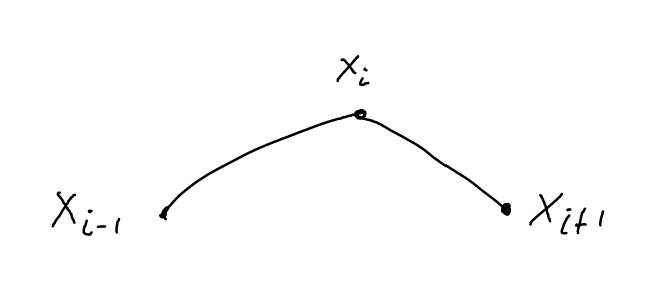
\includegraphics[scale=0.4]{img/base.png}\\
Hay 4 casos posibles:
\begin{enumerate}

\item $x_{i+1} \in \Gamma^+(x_i)$ y $x_i\in \Gamma^+(x_{i-1})$: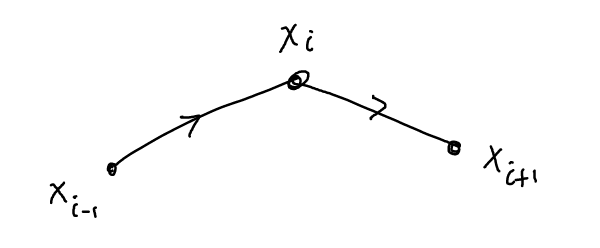
\includegraphics[scale=0.4]{img/forward-forward.png}\\
Como 
\begin{align}
    \left.
    \begin{array}{cc}
    F^*(\overrightarrow{x_i x_{i+1}}) = F(\overrightarrow{x_i x_{i+1}}) + \varepsilon\\
    F^*(\overrightarrow{x_{i-1} x_i}) = F(\overrightarrow{x_{i-1} x_i}) + \varepsilon 
    \end{array}
     \right\} \implies
     \begin{array}{cc}
    out_{F^*}(x_i) = out_F(x_i) + \varepsilon \\
    in_{F*} (x_i) = in_F(x_i) + \varepsilon
    \end{array}
\end{align}
$\therefore out_{F^*} (x_i) - in_{F^*}(x_i) = 0.$\\
Cambiaron los lados que entran y salen de $x_i$.
    
\item $x_{i+1} \in \Gamma^+(x_i)$ y $x_{i-1} \in \Gamma^{-}(x_{i})$: 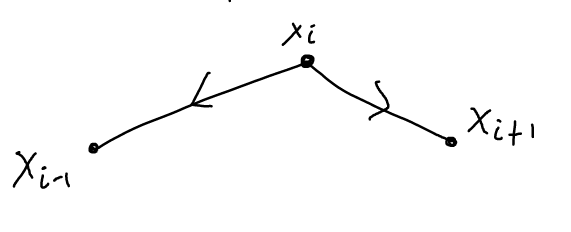
\includegraphics[scale=0.4]{img/backward-forward.png}\\
\begin{align}
    \left.
    \begin{array}{cc}
    F^*(\overrightarrow{x_i x_{i+1}}) = F(\overrightarrow{x_i x_{i+1}}) + \varepsilon\\
    F^*(\overrightarrow{x_{i-1} x_i}) = F(\overrightarrow{x_i x_{i+1}}) - \varepsilon 
    \end{array}
     \right\} \implies
     \begin{array}{cc}
    out_{F^*}(x_i) = out_F(x_i) + \varepsilon -  \varepsilon = out_F(x_i)\\
    in_{F^*} (x_i) = in_F(x_i)
    \end{array}
\end{align}
$\therefore out_{F^*} (x_i) - in_{F^*}(x_i) = 0.$\\
Cambiaron dos lados que salen de $x_i$ y ninguno que entra a $x_i$ cambió.

\item $x_i \in \Gamma^-(x_{i+1})$ y $x_i\in \Gamma^+(x_{i-1}):$ 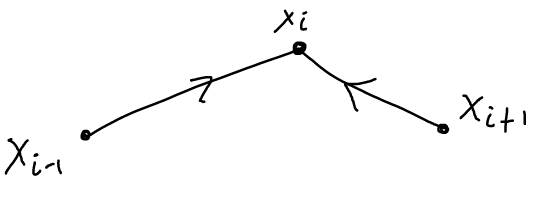
\includegraphics[scale=0.4]{img/forward-backward.png}\\
\begin{align}
    \left.
    \begin{array}{cc}
    F^*(\overrightarrow{x_{i+1} x_i}) = F(\overrightarrow{x_{i+1} x_i}) - \varepsilon\\
    F^*(\overrightarrow{x_{i-1} x_i}) = F(\overrightarrow{x_{i-1} x_i}) + \varepsilon 
    \end{array}
     \right\} \implies
     \begin{array}{cc}
    out_{F^*}(x_i) = out_F(x_i) + \varepsilon -  \varepsilon = out_F(x_i)\\
    in_{F^*} (x_i) = in_F(x_i)
    \end{array}
\end{align}

\item $x_{i}\in \Gamma^-(x_{i+1})$ y $x_{i-1} \in \Gamma^-(x_{i})$: 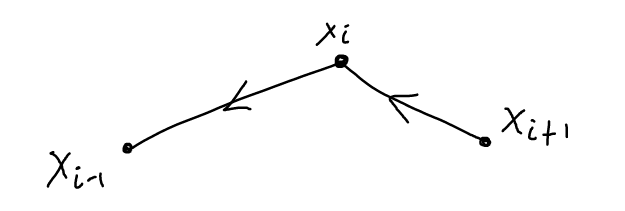
\includegraphics[scale=0.4]{img/backward-backward.png}
\begin{align}
    \left.
    \begin{array}{cc}
    F^*(\overrightarrow{x_i x_{i-1}}) = F(\overrightarrow{x_{i} x_{i-1}}) - \varepsilon\\
    F^*(\overrightarrow{x_{i+1} x_{i}}) = F(\overrightarrow{x_{i+1} x_{i}}) - \varepsilon 
    \end{array}
     \right\} \implies
     \begin{array}{cc}
    out_{F^*}(x_i) = out_F(x_i) + \varepsilon -  \varepsilon = out_F(x_i)\\
    in_{F^*} (x_i) = in_F(x_i)
    \end{array}
\end{align}

\end{enumerate}

Respecto al $v_{F^*}$ tenemos que:\\
Si $x_1 \in \Gamma^+(s)$ entonces
\begin{align}
    V_{F*} &= out_{F^*}(s) - in_{F^*}(s)\\
        &= out_F(s) + \varepsilon - in_{F}(s)\\
        &= v_F + \varepsilon
\end{align}
Si $x_1 \in \Gamma^-(s)$ entonces
\begin{align}
    v_{F^*} &= out_{F^{*}}(s) - in_{F^*}(s)\\
        &= out_F(s) - (in_F(s) - \varepsilon)\\
        &= v_F + \varepsilon
\end{align}
\end{proof}

\begin{lemma}
Sea $N$ un network, $G$ un flujo de $s$ a $t$ y $S$ un corte cualquiera, entonces
\begin{align}
    v_G = G(S, S^c) - G(S^c, S)
\end{align}
\end{lemma}

\begin{proof}
Sea $x\in S$. Vemos que $out_G(x) - in_G(x) = \left\{
    \begin{array}{cc}
     0  &x\neq s\\
     v_G &x = s
    \end{array}
\right.$\\

\begin{align}
    \therefore v_G &= \sum_{x\in S} out(x) - in(x) = \sum_{\substack{x\in S\\xv \in E}} G(x,v) - G(v,x)\\
    &= G(S,V) - G(V,S)  &&\text{Aca usamos: } S \cup S^c = V \wedge S \cap S^c = \varnothing \\
    &= G(S,S) + G(S, S^c) - G(S,S) - G(S^c, S)\\
    &= G(S,S^c) - G(S^c, S)
\end{align}

\end{proof}

\begin{corollary}
El valor del flujo es una cota inferior de la capacidad de un corte $S$ esto es: $v_G \le cap(S)$
\end{corollary}
\begin{proof}
Por restricción de capacidad y conservación, sabemos que \\$G(S, S^c) \le C(S, S^c)$ y $G(S^c, S) \ge 0$ entonces vale:
\begin{align}
v_G &= G(S, S^c) - G(S^c, S)\\
	&\le G(S, S^c)\\
    &\le cap(S)
\end{align}
\end{proof}

\begin{theorem}[\textit{Max-flow min-cut}]
Sea $N = (V,E,C)$ un network, $F$ un flujo de $s$ a $t$ en $N$ y $S$ un corte minimal de $V$ entonces
\begin{align}
    \underbrace{F \text{ es maximal}}_{A} \iff 
    \underbrace{\nexists \text{ caminos } F\text{-aumentantes entre $s$ y $t$}}_{B} \iff
    \underbrace{v_F = mincutcap_S}_{C}
\end{align}
\end{theorem}
\begin{proof}
$C \implies A:$\\
Asumamos $C)$. Sea $S$ un corte con $cap(S) = v_F$\\
Sea $G$ otro flujo. Tenemos por [ref] que
\begin{align} v_G \le cap(S) = v_F \end{align}
de lo que se sigue que $F$ es maximal.\\

Notar que así mismo, $S$ es minimal pues dado un corte cualquiera $T$\begin{align}
    cap(T) \ge v_F = cap(S)
\end{align}
$B \implies C:$\\
Sea $S = \{s\} \cup \{x \in V \mid \exists \text{ camino $F$-aumentante de $s$ a $x$}$\}.
Es claro que $t \notin S$ pues por hipótesis \\$\nexists$ caminos $F$-aumentantes de $s$ a $t$.\\
$\therefore S$ es corte.\\
Como $S$ es corte,
\begin{align}
    v_F = F(S, S^c) - F(S^c, S)
\end{align}
Sea $x \in S$, $y \in S^c$, $\overrightarrow{xy} \in E$. Buscamos $F(xy)$, y vemos que:
\begin{itemize}
    \item $\exists$ un camino F-aumentante $(x_0, x_1,\mathellipsis, x_r)$ entre $s$ y $x$
    \item $\nexists$ un camino $F$-aumentante entre $s$ e $y$
\end{itemize}
Esto es, $(x_0, \mathellipsis, x_r, y)$ no es un camino $F$-aumentante.\\
Como $(x_0, x_1, \mathellipsis, x_r)$ si lo es, y $\overrightarrow{xy} \in E$, concluimos que $\overrightarrow{xy}$ está saturado, ie. \\$F(\overrightarrow{xy}) = C(\overrightarrow{xy})$.
\begin{align}
    \therefore \forall x,y: x \in S \wedge y \in S^c \wedge xy \in E : F(\overrightarrow{xy}) = C(\overrightarrow{xy})\\
    F(S, S^c) = \sum_{\substack{x\in S\\ y \notin S \\\overrightarrow{xy} \in E}} F(\overrightarrow{xy}) = \sum_{\substack{x\in S\\ y \notin S\\ \overrightarrow{xy} \in E}} C(\overrightarrow{xy}) = C(S, S^c) = cap(S)\\
\end{align}
Ahora, veamos el otro caso. Sea $x \in S^c, y \in S, \overrightarrow{xy} \in E$. Buscamos $F(\overrightarrow{xy})$. Con un análisis similar al anterior, teniendo en cuenta que ahora $x\in \Gamma^-(y)$, concluimos $xy$ está vacio ie. $F(\overrightarrow{xy}) = 0$.
\begin{align}
    \therefore \forall x, y : x \in S^c \wedge y \in S \wedge xy \in E : F(\overrightarrow{xy}) = 0\\
    F(S^c, S) = \sum_{\substack{x\not\in S\\ y \in S\\ \overrightarrow{xy} \in E}} F(\overrightarrow{xy}) = \sum_{\substack{x\not\in S\\ y \in S\\ \overrightarrow{xy} \in E}} 0 = 0
\end{align}
Así,
\begin{align}
v_F = F(S, S^c) - F(S^c, S) = cap(S) - 0 = cap(S) = mincutcap_S
\end{align}
Por último, $S$ es claramente minimal.

$A \implies B$:\\
Suponiendo $F$ maximal, supongamos que $B$ es falso, es decir, que existe un camino $F$-aumentante entre $s$ y $t$.\\
Por el lema [\ref{flujo_camino_aumentante}], es posible enviar $\varepsilon$ unidades de flujo por ese camino y obtener un flujo $F^*$ con $v_{F^*} = v_F + \varepsilon$. Esto es absurdo pues $F$ es maximal.
\end{proof}

\begin{algorithm}
\caption{Algoritmo de Edmonds-Karp para hallar flujo maximal}
\begin{algorithmic}
\Require network $N=(V,E,C)$
\Ensure  $(F, v, S)$ donde $F$ es flujo maximal, $v$ es el valor del flujo y $S$ es el corte minimal
\Function{Edmonds-Karp}{$network\ N$}
\State $F = 0, v = 0, \varepsilon(s) = \infty$
\While{$true$} 
    \State $queue\ Q = qEmpty()$
    \State $qEnqueue(Q,s)$
    \State $S := \{s\}$
    \While{$qCnt(Q)$}
        \State $x = qDequeue(Q)$
        \State \ForAll{$z \in \Gamma^{+}(x) \cap S^c$}
        \If{$F(xz) < C(xz)$}
            \State $qEnqueue(Q,z)$
            \State $S = S \cup \{z\}$
            \State $a(z) = x;\ b(z) = 1$
            \State $\varepsilon(z) = min\{\varepsilon(x), C(xz) - F(xz)\}$
        \EndIf
        \EndFor
        \State \ForAll{$z\in \Gamma^{-}(x) \cap S^c$}
        \If{$F(zx) > 0$}
        \State $qEnqueue(Q,z)$
        \State $S = S \cup \{z\}$
        \State $a(z) = x;\ b(z) = -1$
        \State $\varepsilon(z) = min\{\varepsilon(x), F(zx)\}$
        \EndIf
        \EndFor
        \EndWhile
        \State
        \If{$t \in S$}
        \State $q = t;\ \varepsilon = \varepsilon(t);\ v = v+E$
        \While{$q \neq s$}
        \State $p = a(q)$
        \If{$b(q) == 1$}
        \State $F(pq) = F(pq) + \varepsilon$
        \State $F(qp) = F(qp) - \varepsilon$
        \EndIf
        \State q = p;
        \EndWhile
        \Else
        \State \Return{$F, v, S$}
        \EndIf
\EndWhile
\EndFunction
\end{algorithmic}
\end{algorithm}

\begin{theorem}[Teorema de integralidad]\label{integrality}
Sea $N=(V,E,C)$ un network tal que $\forall xy \in E : C(xy) \in \mathbb{Z}$ entonces $\exists$ flujo maximal entero.

En otras palabras, en un network con capacidades enteras encontraremos siempre un flujo maximal entero.
\end{theorem}

\begin{proof}
Lo probaremos por inducción, corriendo el algoritmo de Ford-Fulkerson en $n+1$ pasos, sean $F_0, \mathellipsis, F_n$ los sucesivos flujos obtenidos:\\
Caso base: $F_0 = 0 \in \mathbb{Z}$.\\
Caso inductivo:
$F_k \in \mathbb{Z} \implies F_{k+1} \in \mathbb{Z}$\\
$F_{k+1}$ se construye a partir de $F_k$, cambiando en algunos lados el valor $F_k$ por $F_k \pm \varepsilon$. Por lo tanto, si probamos que $\varepsilon \in \mathbb{Z}$, también tendremos que $F_{k+1} \in \mathbb{Z}$. Luego,
\begin{align}
    \varepsilon = \min\{\epsilon_i\}
\end{align}
y \begin{center}
    $\epsilon_i = \begin{cases} C(\overrightarrow{x_i x_{i+1}}) - F(\overrightarrow{x_i x_{i+1}}) & \text{ si } \overrightarrow{x_i x_{i+1}} \text{ es lado forward}\\
    F(\overrightarrow{x_{i+1} x_i}) & \text{ si } \overrightarrow{x_i x_{i+1}} \text{ es lado backward}
    \end{cases}$
\end{center}
Como las capacidades son todas enteras, $\epsilon_i$ es entero, $\varepsilon$  es entero y por lo tanto $F_{k+1}$.
Esto prueba que si Ford-Fulkerson termina, obtenemos un flujo maximal entero.
Como $v_{F_{k+1}} - v_{F_k} = \varepsilon \in \mathbb{Z} > 0$, por lo tanto $\varepsilon \ge 1$. Esto es, el ``salto" que se produce entre un flujo y el siguiente es discreto.
Como existe una cota superior para el conjunto de valores de flujos posibles (por ej. $cap(S)$), esta sucesión de flujos debe ser finita. 
\end{proof}

\begin{definition}
Dados $a,b\in V$ y un flujo $F$ en un network $N = (V,E,C)$. Definimos a la \emph{distancia (respecto de $\boldsymbol{F}$) de $\boldsymbol{a}$ hasta $\boldsymbol{b}$} como:
\begin{align}
D_F(a,b) = \left\{
    \begin{array}{cc}
         0 & a = b\\
         \#\{x_i x_{i+1} \in E\mid 0\le i < r \}  &\text{si $\{x_0, \mathellipsis, x_r\}$ es el menor camino $F$-aumentante entre $a$ y $b$} \\ 
         \infty &\text{si $\nexists$ camino $F$-aumentante entre $a$ y $b$}
    \end{array}
    \right.
\end{align}
Esto es, el numero de lados del menor camino aumentante relativo a $F$ entre $a$ y $b$.\\
Asimismo, definimos
\begin{itemize}
    \item $d_F(x) \doteq D_F(s,x)$
    \item $b_F(x) \doteq D_F(x,t)$
\end{itemize}
\end{definition}

\begin{lemma}\label{distancias_no_decrecen_EK}
Sea $N=(V,E,C)$ un network y $F_1, F_2, \mathellipsis, F_\ell$ los flujos parciales obtenidos por Edmonds-Karp (supongamos que $F_0 = 0$ es el flujo inicial).\\
Abreviaremos
\begin{align}
    d_k(x) \doteq d_{F_k}(x) \\
    b_k(x) \doteq d_{F_k}(x)
\end{align} entonces tenemos que $\forall x \in V$:
\begin{align}
    d_k(x) \le d_{k+1}(x) \\
    b_k(x) \le b_{k+1}(x)
\end{align}
\end{lemma}

\begin{proof}
$\forall i : 1 \le i \le \ell$ :\\
\begin{enumerate}
    \item
    Sea $A_i \doteq \{x \in V \mid d_i(x) < d_{i-1}(x)\}$, queremos ver que $A_i = \varnothing$ comenzando por notar que $s \notin A_i$ ya que $\forall i: d_i(s) = 0$.\\
    Supongamos que $\exists i : A_i \neq \varnothing$. Sea ese $i$ el mínimo posible. A su vez, sea $x = \min\{d_i(v) \mid v \in A_i \}$, ie. tal que $d_i(x)$ sea mínimo. Entonces, $\forall z : d_i(z) > d_i(x) \implies z\notin A_i$.\\
    Como $d_i(x) < d_{i-1}(x) \le \infty$ tenemos que $d_i(x) < \infty$ y debe haber un camino $F_i$-aumentante de $s$ a $x$. Sea $(x_0, \mathellipsis, x_r)$ el camino mínimo (es decir, con $r = d_i(x)$).\\
    Probemos ahora que $\nexists$ un camino $F_{i-1}$-aumentante de $s$ a $x$, y luego lleguemos a una contradicción.\\
    Sea $z = x_{r-1}$. Como $(x_0,\mathellipsis, x_r)$ es el camino $F_i$-aumentante de menor longitud entre $s$ y $x$ entonces $(x_0, \mathellipsis, x_{r-1})$ es el camino $F_{i}$-aumentante de menor longitud entre $s$ y $z$. Así, como $d_i(z) = r-1$ se sigue que $z \notin A_i$. Concluimos que $d_{i-1}(z) \le d_i(z) < d_i(x) < d_{i-1}(x)$. \\
    $\therefore d_{i-1}(z) \le d_{i-1}(x)-2$.
    Pero consideremos que $d_{i-1}(x) \le d_{i-1}(z) + 1$, ya que se puede ir de $z$ a $x$.
    Como $d_{i-1}(z)+2 \le d_{i-1}(x)$, esto es absurdo.\\
    $\therefore \nexists$ camino $F_{i-1}$-aumentante $(s,\mathellipsis, z, x).$\\
    Ahora la contradicción:\\
    Como existe un camino $(s, \mathellipsis, z, x)$, debe pasar $x \in \Gamma^+(z)$ o bien $x \in \Gamma^-(z)$. La razón por la que no existe un camino $F_{i-1}$ aumentante puede ser alguna de las siguientes:
    \begin{itemize}
        \item $x \in \Gamma^+(z) \wedge F_{i-1}(\overrightarrow{zx}) = C(\overrightarrow{zx})$
        \item $x \in \Gamma^-(z) \wedge F_{i-1}(\overrightarrow{zx}) = 0$ 
    \end{itemize}
    Pero como el camino $F_i$-aumentante si existe,
    \begin{itemize}
        \item $x \in \Gamma^+(z) \wedge F_{i-1}(\overrightarrow{zx}) = C(\overrightarrow{zx}) \wedge F_i(\overrightarrow{zx}) < C(\overrightarrow{zx})$
        \item $x \in \Gamma^-(z) \wedge F_{i-1}(\overrightarrow{zx}) = 0 \wedge F_i(\overrightarrow{zx}) > 0$
    \end{itemize}

    La única forma en que esto puede ocurrir es que al pasar de $F_{i-1}$ a $F_i$ usemos un camino de la forma $(s, \mathellipsis, x, z)$, ya que:
    \begin{itemize}
        \item Si el último lado es backward, $x \in \Gamma^+(z) \wedge F_{i}(\overrightarrow{zx}) < F_{i-1}(\overrightarrow{zx})$ (primer razón).
        \item Si el último lado es forward, $x \in \Gamma^-(z) \wedge F_{i}(\overrightarrow{xz}) > F_{i-1}(\overrightarrow{xz})$ (segunda razón).
    \end{itemize}
    Como usamos Edmonds-Karp, este camino tiene longitud mínima.
    Entonces $d_{i-1}(z) = d_{i-1}(x) + 1$. Pero sabemos que $d_{i-1}(x) + 1  = d_{i-1}(z) \le d_{i-1}(x) - 2$. Esto es una contradicción. Concluimos:
    \begin{align}
        \nexists i : A_i \neq \varnothing
        \equiv
        \forall i : A_i = \varnothing
    \end{align}
    Es decir, $\forall i, x : x \in V : d_{i-1}(x) \le d_i(x)$
    \item
    Similarmente, podemos construir un $B_i = \{x \in V \mid b_i(x) < b_{i-1}(x) \wedge i \ge 1\}$ y probar que
    \begin{align}
    \forall i : B_i = \varnothing && \text{ie.}\\
    \forall i, x : x \in V : b_{i-1}(x) \le b_i(x)
    \end{align}
    \end{enumerate}
\end{proof}

\begin{theorem}[Complejidad del algoritmo de Edmonds-Karp] 
El algoritmo de Edmonds-Karp para encontrar un flujo maximal y un corte minimal en un network es de complejidad $\mathcal{O}(n m^2)$
\end{theorem}
\begin{proof}
Notemos que al construir cada $F_i$ pasa una de las siguientes:
\begin{itemize}
    \item Al menos un lado forward se satura.
    \item Al menos un lado backward se vacía.
\end{itemize}
Llamamos \emph{crítico} a un tal lado.
Supongamos que un lado con vértices $x$ y $z$ se volvió crítico en el paso $i$. Antes de que pueda volverse crítico deberá usarse para el otro lado (si se usó como forward, debe usarse como backward, y viceversa). Supongamos que sucede eso en el paso $j > i$.\\
Así, $(s, \mathellipsis, z, x)$ es un camino mínimo en el paso $i$, y $(s,\mathellipsis, x, z)$ en el paso $j$.
Como el camino $F$-aumentante de $s$ a $t$ en el paso $j$ contiene a $z$:
\begin{align}
    d_j(t) = d_j(z)+b_j(z)
    \end{align}
Además, $z$ está después de $x$ en este camino:
\begin{align}
    d_j(t) = d_j(x) + 1 + b_j(z)
\end{align}
Por el lema [\ref{distancias_no_decrecen_EK}], sabemos que $d_{i-1}(x) \le d_i(x)$ (haciendo la sustitución: $i-1 := i \wedge i := j$) y:\begin{align}
    d_j(t) \ge d_i(x) + 1 + b_i(z)
\end{align}
Y ahora, en el paso $i$, $z$ está antes que $x$:
\begin{align}
    d_j(t) \ge d_i(x) + 1 + 1 + b_i(x)
\end{align}
Y entonces:
\begin{align}
    d_j(t) \ge d_i(t) + 2
\end{align}
Concluimos que si un lado se vuelve crítico, antes de que pueda volver a hacerlo, la distancia entre $s$ y $t$ debe aumentar en al menos $2$.\\
Por lo tanto, un lado puede volverse crítico a lo sumo $\frac{n+1}{2} \in \mathcal{O}(n)$ veces.
Sabemos que en la construcción de cada $F_i$ al menos un lado se vuelve crítico. Así, tenemos que \begin{align}
    \# F_i &\le m * \# \text{veces que puede volverse crítico}\\
    \# F_i &\in \mathcal{O}(nm)
\end{align}
Cada corrida consiste en construir un $F_i$ mediante $BFS \in \mathcal{O}(m)$.\\
 $\therefore$ La complejidad del algoritmo Edmonds-Karp es $\mathcal{O}(m) * \mathcal{O}(nm) = \mathcal{O}(nm^2)$
\end{proof}

\subsection{Dinic-Even}

\begin{algorithm}
\caption{Algoritmo de Dinic-Even para encontrar flujo maximal}
\begin{algorithmic}
\Require network $N=(V,E,C)$
\Ensure  $F$ un flujo maximal
\Function{Dinic}{$network\ N$}
\State $F = 0$
\State $L$ = \Call{LayeredNetwork}{$N, F$} \Comment{ Construir un network auxiliar por niveles $L$ basado en $F$ y $N$}
\While{$t \notin L$}
    \State $F$ += \Call{BlockingFlow}{$L$}
    \State $L$ = \Call{LayeredNetwork}{$N, F$}
\EndWhile
\State \Return{$F$}
\EndFunction

\State

\Function{BlockingFlow}{layered network $L$}
\State $len = d_L(s,t)$
\State vertex path $P = [s]$
\State $G = 0$ \Comment{Este será flujo bloqueante}
    \While{$true$}
    \State $i = 0$
        \While{$i < len$}
            \State $v = P[i]$
            \If{$\Gamma^+(v) \neq \varnothing$}
                \Comment{Avanzar}
                \State $P$ += algún vecino de $v$
                \State $i$ += $1$
            \ElsIf{$v \neq s$}
                \Comment{No podemos llegar a $t$: Retroceder}
                \State $E_L$ -= $\overrightarrow{P[i-1] P[i]}$
                \State $i$ -= $1$
            \Else
                \State \Return{$G$} \Comment{Solo terminamos cuando $\Gamma^+(s) = \varnothing$}
            \EndIf
        \EndWhile
    
        \Comment{Llegamos a $t$: Incrementar}
        \State $\varepsilon = \min_{0\le i < len} \{ C(\overrightarrow{P[i] P[i+1]}) - G(\overrightarrow{P[i] P[i+1]})\}$
        \For {$i \in \{0, \mathellipsis, len-1\}$}
            \State $G(\overrightarrow{P[i] P[i+1]})$ += $\varepsilon$
            \If {$C(\overrightarrow{P[i] P[i+1]}) = G(\overrightarrow{P[i] P[i+1]})$}
                \State $E_L$ -= $\overrightarrow{P[i] P[i+1]}$
            \EndIf
        \EndFor
    \EndWhile
\EndFunction
\end{algorithmic}
\end{algorithm}

\begin{definition}[Network por niveles]
Un network $N = (V,E,C)$ es un \emph{network por niveles} si:
\begin{align}
 V &= \bigcup_{i=0}^r V_i \\
 E &= \{\overrightarrow{xy} \mid \forall i: 0 \le i \le r : x \in V_i \wedge y \in V_{i+1}\}
 \end{align}
 tal que $\forall i, j : 0 \le i < j \le r \wedge i \neq j : V_i \cap V_j = \varnothing$ \\
Y con $V_0 = \{s\} \text{ y } V_r = \{t\}$

Es decir, solo hay lados entre vértices de distintos niveles siendo el primer nivel el de $s$ y el último el de $t$.
\end{definition}

\begin{definition}[Network residual]
Dado un network $N = (V_N, E_N, C_N)$ y un flujo $F_N$, el \emph{network residual} $R$ = $R_F$ = $R_{F_N} = (V_R, E_R, C_R)$ es el network tal que:
\begin{itemize}
    \item $V_R = V_N$
    \item $(\overrightarrow{xz}) \in E_R \iff 
    \left\{ 
    \begin{array}{cc}
    \overrightarrow{xz} \in E_N \wedge F_N(\overrightarrow{xz}) < C_N(\overrightarrow{xz})     & \text{caso \textit{forward}} \\
    \text{o bien}  & \\
    \overrightarrow{zx} \in E_N \wedge F_N(\overrightarrow{zx}) > 0 & \text{caso \textit{backward}}
    \end{array}
    \right.$
    \item $C_R(\overrightarrow{xz}) = \left\{
    \begin{array}{cc}
        C_N(\overrightarrow{xz}) -
        F_N(\overrightarrow{xz})   & \text{caso \textit{forward}}\\
        F_N(\overrightarrow{zx})   & \text{caso \textit{backward}}
    \end{array}
    \right.
    $
\end{itemize}
\end{definition}

\begin{definition}[Network auxiliar por niveles o \textit{level graph}]
Dado un network residual $R = R_F = R_{F_N} = (V_R, E_R, C_R)$ definimos al \emph{network auxiliar por niveles} o $\boldsymbol{level}$  $\boldsymbol{graph}\ L = L_F = (V_L, E_L, C_L)$ de la siguiente forma:
\begin{itemize}
    \item $V_L = \{ x\in V_R \mid d_F(x) < d_F(t)\} \cup \{t\}$
    \item $E_L = \{\overrightarrow{xy} \in E_R \mid d_F(x) + 1 = d_F(y)$\}
    \item $C_L = C_R$
\end{itemize}

\end{definition}

\begin{definition}[Flujo bloqueante]
Un \emph{flujo bloqueante} o $\boldsymbol{blocking}$  $\boldsymbol{flow}$ es un flujo tal que todos los caminos dirigidos de $s$ a $t$ tienen al menos un lado saturado.
\end{definition}

\begin{algorithm}
\caption{Pseudocódigo de Algoritmos tipo Dinic}
\begin{algorithmic}
\State $F = 0$
\While{$d_F(t) < \infty$}
    \State Construir un \textit{level graph} $L = L_F$
    \State Hallar flujo bloqueante $G$ en $L$
    \State Modificar $F$ en $N$ de acuerdo a $G$
\EndWhile

\end{algorithmic}
\end{algorithm}

\begin{theorem}
Entre dos level graphs consecutivos la distancia entre $s$ y $t$ aumenta.
\end{theorem}

\begin{proof}
Sean $A$ y $B$ dos networks auxiliares consecutivos. Probaremos que $d_A(t) < d_B(t)$. 
Sabemos que $d_A(t) \le d_B(t)$ por el lema [\ref{distancias_no_decrecen_EK}] de Edmonds-Karp (seguimos utilizando el camino más corto).
Debemos entonces probar que $d_A(t) \neq d_B(t)$.\\
Primero, observemos que $s, x_1, \mathellipsis, x_{r-1}, t$ es un camino dirigido no saturado en $A \iff$ no lo es en $B$, puesto que si es no saturado en $A$ el flujo bloqueante satura uno de sus lados, y si no lo es en $B$ entonces no estaba en $A$ (el flujo bloqueante lo hubiera saturado).\\
Sea $s, x_1, \mathellipsis, x_{r-1}, t$ el mínimo camino dirigido no saturado en $B$. Como dijimos, este camino no estaba en $A$. Esto puede darse por dos razones:

\begin{enumerate}
    \item Caso 1: $\exists i : x_i \in V_B : x_i \notin V_A$: Falta un vértice $x_i$ en $A$ que si está en el $B$ (notar que $x_i \neq s,t$).\\
    Entonces $d_A(t) \le d_A(x_i)$, ya que si la distancia fuese menor hubiera estado en $A$. Por el lema de E-K [\ref{distancias_no_decrecen_EK}], $d_A(x_i) \le d_B(x_i)$.\\
    Así, $d_{A}(t) \le d_{A}(x_i) \le d_{B}(x_i) < d_{B}(t)$ ($x_i$ está antes de $t$ en el camino en $B$). Así, $d_A(t) < d_B(t)$.
    
    \item Caso 2: $\exists i : \overrightarrow{x_{i-1} x_i} \notin E_A$: falta un lado $\overrightarrow{x_{i-1} x_{i}}$ pero ningún vértice. 
    Esto puede pasar por dos razones (correspondientes a la definición de $E_R$ y $E_A$). \\
    Tomemos el mínimo $i$ tal que $\overrightarrow{x_{i-1} x_{i}} \notin E_A$:
    
    \begin{enumerate}
    \item Caso A: El lado está saturado o vacío (en $N$).\\
    Como en $E_B$ este lado si está, al incrementar el flujo en $A$ debimos usarlo en el otro sentido: con un camino $s, \mathellipsis, x_i, x_{i-1}, \mathellipsis, t$. Así,
    \begin{align}
        d_B(t)
        &= d_B(x_i) + b_B(x_i)\\
        &= d_B(x_{i-1}) + 1 + b_B(x_i)\\
        &\ge d_A(x_{i-1}) + 1 + b_A(x_i)\\
        &\ge d_A(x_{i-1}) + 1 + b_A(x_{i-1}) + 1\\
        &\ge d_A(t) + 2\\
        &> d_A(t)
    \end{align}
    Como en E-K.
    %$\left.
    %\begin{array}{cc}
    %(\overrightarrow{x_{i-1} x_{i}}) \notin  E_{R_{A}}     &  \\
    %(\overrightarrow{x_{i-1} x_{i}}) \in E_{R^*_{B}}     & 
    %\end{array}
    %\right\}$
    %solo puede ocurrir si $(\overrightarrow{x_{i} x_{i-1}}) \in E_L$\\
    %Veamos lo anterior:\\
    %Supongamos que 
    %$(\overrightarrow{x_{i+1} x_i}) \in E_L$, luego $d_A(x_{i+1}) + 1 = d_A(x_i)$\\
    %Entonces, $d_A(t) = d_A(x_i) + b_A(x_i)$. Pero $\overrightarrow{(x_i x_{i+1}})$ es el primer %lado que no está en $E_L$
    %\begin{align}
    %\forall k : 0 \le k < i &: (\overrightarrow{x_{k-1} x_{k}}) \in E_L \implies \\
    %\forall j : j < i &: d_A(x_j) = j 
    %\end{align}
    %Entonces, $(\overrightarrow{x_{i-1} x_{i}}) \notin E_{R_A} \wedge (\overrightarrow{x_{i-1} x_{i}}) \in E_{R^{*}_B}$
         
    \item Caso B: El lado no está saturado ni vacío: $d_A(x_i) + 1 \neq d_A(x_{i-1})$\\
    Esto significa que $d_A(x_{i}) \le d_A(x_{i-1}) + 1$ (si no, como el lado no esta saturado ni vacío, estaría en $E_A$).
    $\therefore d_A(x_i) < d_A(x_{i-1}) + 1$. Como el camino es mínimo en $B$,
    \begin{align}
        d_B(t)
        &= d_B(x_i) + b_B(x_i)\\
        &= d_B(x_{i-1}) + 1 + b_B(x_i)\\
        &\ge d_A(x_{i-1}) + 1 + b_A(x_i)\\
        &\ge d_A(x_i) + 1 + b_A(x_i)\\
        &\ge d_A(t) + 1\\
        &> d_A(t)
    \end{align}
    %Pero $d_A(x_{i-1}) = i-1$ (pues $\forall j < i : d_A(x_j) = j$\\
    %Por lo tanto, $d_A(x_{i}) \neq  i-1 +1 = i$, pero como $d_A(x_{i}) \le d_B(x_{i}) = i$, 
    %tenemos que $d_A(x_{i}) < i$\\
    %$\therefore d_A(t) = d_A(x_{i}) + b_A(x_{i}) < i + b_A(x_{i}) \le i + b_B(x_{i}) = d_B(x_{i}) + b_B(x_{i}) = d_B(t)$\\
    %$\therefore d_A(t) < d_B(t)$
    \end{enumerate}
    %Volviendo al caso $A$, tenemos que $d_A(x_i) + 1 = d_A(x_{i-1}) = i-1$\\
    %$\therefore d_A(x_i) = i - 2 < i$ y vale la prueba de 2B.
\end{enumerate}
\end{proof}

\begin{theorem}
La complejidad del paso de flujo bloqueante en el algoritmo de Dinic-Even es $\mathcal{O}(nm)$
\end{theorem}
\begin{proof}
Sean \begin{itemize}
    \item A := 'Avanzar'
    \item R := 'Retroceder'
    \item I := 'Incrementar $G$'
\end{itemize}
Una corrida se corresponde a:
$A^*(A^*R^*)^*I$.\\
Consideremos entonces las palabras de la forma $A^*x$ (con $x \in \{ R, I \}$).
Necesitamos saber cuántas palabras hay y cuál es la complejidad de cada una.
Tengamos en cuenta lo siguente:
\begin{itemize}
    \item $compl$(A) = $\mathcal{O}(1)$
    \item $compl$(R) = $\mathcal{O}(1)$
    \item $compl$(I) = $\mathcal{O}(n)$. 
\end{itemize}

Teniendo en cuenta que R borra un lado del \textit{level graph} y que I también borra al menos un lado (pues al incrementar el flujo se satura al menos un lado) tenemos que:
\begin{align}
    \#palabras(A^*x) \le m
\end{align}

Veamos ahora la complejidad de cada palabra:
\begin{align}
\underbrace{A\mathellipsis A}_j R &\rightarrow \underbrace{\mathcal{O}(1)+\mathellipsis+\mathcal{O}(1)}_j+ \mathcal{O}(1) = \mathcal{O}(j)\\
\underbrace{A\mathellipsis A}_j I &\rightarrow \mathcal{O}(j) + \mathcal{O}(n)
\end{align}
Estamos en un \textit{level graph} y A mueve el pivot $p$ desde $p$ hasta un vecino de $p$. Por lo tanto, A incrementa en 1 el nivel de $p$. Luego de a lo sumo $n$ Avanzar debo llegar a $t$ (o se produce un I o bien hay que Retroceder). Luego $j \le n$

\begin{align}
    \therefore compl(\text{A...AR}) &= \mathcal{O}(j) = \mathcal{O}(n)\\
    compl(\text{A...AI}) &= \mathcal{O}(j) + \mathcal{O}(n)\\
    &= \mathcal{O}(n) + \mathcal{O}(n)\\
    &= \mathcal{O}(n)
\end{align}

Conclusión: $\# palabras \in \mathcal{O}(m)\ \wedge \  compl(palabra) \in \mathcal{O}(n) \implies$
Complejidad del paso de flujo bloqueante del algoritmo de Dinic-Even es $\mathcal{O}(nm)$

\end{proof}

\begin{theorem}
La complejidad del algoritmo de Dinic-Even es $\mathcal{O}(n^2 m)$
\end{theorem}
\begin{proof}
En [ref] vimos que la distancia de $s$ a $t$ en level graphs consecutivos aumenta.\\
$\therefore$ Hay a lo sumo $n-1$ \textit{level graphs}.\\
Tambien vimos que la complejidad del paso bloqueante es $\mathcal{O}(nm)$.
\end{proof}

\begin{definition}
Un network $N = (V,E,C)$ se dice unitario si tiene capacidad $1$ en todos sus lados.\\
$\forall \overrightarrow{xy} \in E : C(\overrightarrow{xy}) = 1$ \\
$\forall x \neq s,t : |\Gamma^+(x)| = 1 \veebar |\Gamma^-(x)| = 1$
\end{definition}
\begin{theorem}
Dinic en un network unitario tiene complejidad $\mathcal{O}(m\sqrt{n})$
\end{theorem}

\begin{proof}
Supongamos que hago $\sqrt{n}$ flujos bloqueantes y el algoritmo aún no termina.
Sea $F$ el flujo que tenemos. Notemos que $F \in \mathbb{Z}$ y que $R_F$ es unitario:
\begin{itemize}
    \item Si $F < C$, $C' = 1$
    \item Si no, $C' = F = 1$
\end{itemize}
Sea $G$ el flujo maximal en $R_F$ obtenido por Dinic.
Como es flujo, $\forall x \neq s,t : out_G(x) = in_G(x)$
Como $C' \le 1$:
\begin{itemize}
    \item si $|\Gamma^-(x)| = 1, in_G(x) \le 1$, es decir $in_G(x) = 0$
\end{itemize}
\end{proof}

\subsection{Wave}
En Edmonds-Karp y Dinic el invariante es que $F$ es flujo, el algoritmo transforma un flujo en otro, y se detiene cuando no hay mas caminos aumentantes (E-K) o no hay mas caminos bloqueantes (Dinic).
Varios algoritmos invierten el esquema: se parte de un pseudo-flujo bloqueante, se lo va transformando en otros pseudo-flujos bloqueantes, hasta obtener un flujo propiamente dicho.

Wave: como $MKM$ pero desde $s$.
Veamos el paso bloqueante:
Sea $(x_0 = s, x_1, \mathellipsis, x_r = t)$ es el orden $BFS$ de la construcción de este network auxiliar.
\begin{algorithm}
\begin{algorithmic}
\Function{Paso bloqueante de Wave}{network N}
\State $G  = 0$
\For{$x\in V$}
\State $D(x) = 0$ \Comment{desbalance in-out}
\EndFor
\For{$x \neq s \wedge x\in V$}
\State $D(x) = 0$
\EndFor
\For{$x \neq s \wedge x \in V$} 
\State $B(x) = false$ \Comment{vértice bloqueado}
\State $A(x) = \varnothing$ \Comment{vértices que le mandan}
\EndFor
\For{$x \in \Gamma^+(s)$}
\State $G(\overrightarrow{sx}) = C(\overrightarrow{sx})$
\State $D(x)$ += $C(\overrightarrow{sx})$
\State $D(s)$ -= $C(\overrightarrow{sx})$
\State $A(x) = \{s\}$
\EndFor
\While{$D(s) + D(t) \neq 0)$}
\For{$x \in [x_1,\mathellipsis,x_{r-1}]$} \Comment{forward wave}
\If{$D(x) > 0$}
\State{$\Call{forwardBalance}{x}$}
\EndIf
\EndFor
\For{$x \in [x_{r-1} \mathellipsis, x_1]$} \Comment{backward wave}
\If{$D(x) < 0 \wedge B(x)$}
\State{$\Call{backwardBalance}{x}$}
\EndIf
\EndFor
\EndWhile
\EndFunction
\end{algorithmic}
\end{algorithm}

\begin{algorithm}
\begin{algorithmic}
\Function{forwardBalance}{vertex x}
\While{$D(x) > 0 \wedge \Gamma^+(x) \neq \varnothing$}
\State elegimos $z \in \Gamma^+(x)$
\If{B(z)}
\State{$\Gamma^+(x) := \Gamma^+(x) - \{z\}$}
\Else
\State $m = min\{D(x), C(\overrightarrow{xz}) - G(\overrightarrow{xz})\}$
\State $G(\overrightarrow{xz}$ += $m$
\State $D(x)$ -= $m$
\State $D(z)$ += $m$
\State $A(z) = A(z) \cup \{x\}$
\If{$G(\overrightarrow{xz}) == C(\overrightarrow{xz})$}
\State $\Gamma^+(x) := \Gamma^+(x) - \{z\}$
\EndIf
\If{$D(x) > 0$}
\State $B(x) := true$
\EndIf
\EndIf
\EndWhile
\EndFunction
\end{algorithmic}
\end{algorithm}

\begin{algorithm}
\begin{algorithmic}
\Function{backwardBalance}{vertex x}
\While{$D(x) > 0$}
\State elegimos $z \in A(x)$
\State $m = min\{D(x), G(\overrightarrow{zx})\}$
\State $G(\overrightarrow{zx}$ -= $m$
\State $D(x)$ -= $m$
\State $D(z)$ -= $m$
\If{$G(\overrightarrow{zx}) == 0$}
\State $A(x) := A(x) - \{z\}$
\EndIf
\EndWhile
\EndFunction
\end{algorithmic}
\end{algorithm}

\begin{theorem}
La complejidad del algoritmo de Wave es $\mathcal{O}(n^3)$
\end{theorem}

\begin{proof}
Wave es de tipo Dinic. Tiene $\mathcal{O}(n)$ networks auxiliares. Probemos que el paso bloqueante es $\mathcal{O}(n^2)$
Al correr el paso bloqueante hacemos una serie de \Call{forwardBalance}{x} y \Call{backwardBalance}{x}.
Al hacer \Call{ForwardBalance}{x} procesamos lados $\overrightarrow{xz}$ de dos categorias posibles:
\begin{itemize}
    \item Categoría T(otal): al procesarlo, $G(\overrightarrow{xz}) = C(\overrightarrow{xz})$. Es decir, se satura o vacía el lado.
    \item Categoría P(arcial): al procesarlo, $G(\overrightarrow{xz}) < C(\overrightarrow{xz})$
\end{itemize}
En los T se remueve de $\Gamma^+(x)$. Solo se entra una vez a T.
El total de lados de categoria T sobre todos los \Call{forwardBalance} sobre todos las olas es $\mathcal{O}(m)$.
De los de categoría P hay a lo sumo uno en cada \Call{forwardBalance}{x}:

$\#$ lados en cat P $\le \#FB$ totales.\\
En una ola hacia adelante hay a lo sumo $(n-2)$ FB(x).
En una de estas olas, puede pasar:
\begin{itemize}
    \item Todos los vértices quedan balanceados.
    \item Queda alguno no balanceado.
\end{itemize}
Toda ola bloquea al menos un vértice.
Como los vértices nunca se desbloquean, hay $\mathcal{O}(n)$ olas hacia adelante.\\
Entonces:
\begin{align}
\#FB &\le (n-2) \# olas
     \le (n-2) \mathcal{O}(n) = \mathcal{O}(n^2)
\end{align}

\text{Complejidad de todos las olas hacia adelante} = \# lados tipo T + \# lados tipo P\\
= $\mathcal{O}(m) + \mathcal{O}(n^2) = \mathcal{O}(n^2)$

Olas hacia atrás:
En los BB(x) también hay dos categorias:\begin{itemize}
    \item T: $G(\overrightarrow{zx})  = 0$
    \item P: $G(\overrightarrow{zx}) > 0$
\end{itemize}
Hay a lo sumo uno de tipo $P$ en cada BB(x).\\
$\#$ tipo P $\le \#$ BB(x)
$\le \mathcal{O}(n) \cdot \#$ olas hacia atras \\
$\le \mathcal{O}(n) \cdot \#$ olas hacia adelante
$\le \mathcal{O}(n) \cdot \mathcal{O}(n)$\\

Tipo T:
Si $\overrightarrow{zx}$ es de tipo T, $z$ se remueve de $A(x)$
¿Cuántas veces puedo agregar a $z$ a $A(x)$ luego de esto?
Necesito que $z$ le mande flujo a $x$ para que pase.
Pero solo hacemos BB(x) si $x$ está bloqueado y si $x$ está bloqueado, como nunca se desbloquea, $z$ no le puede mandar flujo.\\
Así, hay a lo sumo $m$ lados de tipo T y $\#$ olas hacia atrás $\le \#$ tipo T $+ \#$ tipo P
$\le \mathcal{O}(m) + \mathcal{O}(n^2)
\le \mathcal{O}(n^2)$
\end{proof}

\begin{lstlisting}[language=Python]
# levels = [lvl_1, ...., lvl_r]
# where lvl_k contains vertices in the k-th level
# and lvl_0 = [s], lvl_r = [t]
def blockingFlow(AN):
    vs = concat(levels)
    D(s) = CAP({s})
    FB(s)
    while D(s) + D(t) is not 0:
        for v in vs if not B(v):
            FB(v)
        for v in reverse(vs) if B(v):
            BB(v)

def FB(v):
    for w in FNeighbours(v) if D(v) > 0:
        if B(w) or g(v,w) is c(v,w):
            continue
        m = min(D(v), c(v,w)-g(v,w))
        g(v,w) += m
        D(v) -= m
        D(w) += m
    if D(v) > 0:
        B(v) = true
        
def BB(v):
    for w in BNeighbours(v) if D(v) > 0:
        if g(w,v) is 0:
            continue
        m = min(D(v), g(w,v))
        g(w,v) -= m
        D(v) -= m
        D(w) += m
\end{lstlisting}
%\pagebreak

%\section{Matchings en grafos bipartitos}
%\begin{definition}
Dado un grafo $G$, un \emph{matching}, \emph{apareamiento} o \emph{emparejamiento} en $G$ es un subgrafo M de G tal que 
\begin{align}
    \forall x\in V_M :: \exists! y\in V_M : xy \in E_M
\end{align}
\end{definition}

\begin{definition}
Un matching M es \emph{perfecto} si $\left| V_M \right| = \left| V_G \right|$.\\
Un matching $M$ en $G$ es \emph{maximal} si $\nexists~ l \in E_G : (V_M, E_M \cup \{l\})$ es matching.\\
Un matching $M$ en $G$ es \emph{máximo} si $\forall M'$ matching en $G : |E_{M'}| \le |E_M|$.\\
Notar además que $M$ perfecto $\implies M$ máximo, y $M$ máximo $\implies M$ maximal.
\end{definition}

Restringimos nuestro estudio a hallar matchings máximos en grafos bipartitos, a los que denotaremos $G = (\mathcal{X} \cup \mathcal{Y}, E)$.

\begin{theorem}[Isomorfismo entre flujos enteros y matchings]
Hallar un matching en un grafo bipartito y hallar un flujo en un network son equivalentes.
\end{theorem}
\begin{proof}
Sea $G = (\mathcal{X} \cup \mathcal{Y}, E)$ un grafo bipartito.
Definiremos un network $N$ tal que dado un flujo en $N$, podamos construir un matching en $G$, y que dado un matching en $G$, podamos construir un flujo en $N$.
Sean
\begin{align}
    V_N &= V_G \cup \{s,t\} && s,t\notin V_G\\
    E_N &= \{\overrightarrow{sx} \mid x\in \mathcal{X}\} 
    \cup 
    \{\overrightarrow{xy} \mid x\in\mathcal{X} \wedge y\in\mathcal{Y} \wedge \overrightarrow{xy} \in E_G\}
    \cup 
    \{\overrightarrow{yt} \mid y\in \mathcal{Y}\}\\
    C_N (l) &= 1 && \forall l \in E_N
\end{align}

Sea $M$ un matching en $G$. Definimos $F_M$ la siguiente función sobre los lados de $N$:
\begin{align}
    F_M(\overrightarrow{xy}) &=
    \left\{
    \begin{array}{cc}
          1 & \mid xy \in E_M\\
          0 & \mid xy \notin E_M
    \end{array}\label{edges}
    \right. \\
    F_M(\overrightarrow{sx}) &= 
    \left\{
    \begin{array}{cc}
        1  & \mid x \in V_M\\
        0  & \mid x \notin V_M
    \end{array}\label{edges_s}
    \right. \\
    F_M(\overrightarrow{yt}) &=
    \left\{
    \begin{array}{cc}
        1  &\mid y \in V_M\\
        0  &\mid y \notin V_M
    \end{array}\label{edges_t}
    \right.
\end{align}

Probemos que $F_M$ es un flujo de $s$ a $t$ en $N$.
\begin{enumerate}
    \item Restricción de capacidad: Es obvio que $\forall l \in E_N : 0 \le F_M(l) \le 1$.
    \item Conservación: Sea $z \neq s,t$.
    \begin{enumerate}
        \item Si $z \in \mathcal{X}$, $\Gamma^-(z) = {s}$, $in_{F_M}(z) \le 1$.
        \begin{itemize}
            \item Si $in_{F_M}(z) = 0 \implies F_M(\overrightarrow{sz}) = 0 \implies z \notin V_M \implies \nexists y \in \mathcal{Y} : zy \in E_M \implies \forall y \in \mathcal{Y} : F_M(\overrightarrow{zy}) = 0 \implies out_{F_M}(z) = 0$
            \item Si $in_{F_M}(z) = 1 \implies F_M(\overrightarrow{sz}) = 1 \implies z \in V_M \implies \exists! y \in \mathcal{Y} : zy \in E_M \implies \exists! y \in \mathcal{Y} : F_M(\overrightarrow{zy}) = 1 \implies out_{F_M} = 1$
        \end{itemize}
        \item Si $z \in \mathcal{Y}$, $\Gamma^+(z) = {t}$, $out_{F_M}(z) \le 1$. Un análisis similar al anterior vale.
    \end{enumerate}
    \item La fuente es productora. Como $\Gamma^-(s) = \varnothing$, $in_{F_M}(s) = 0$ y $in_{F_M}(z) \le out_{F_M}(z)$.
    \item El resumidero es consumidor. Como $\Gamma^+(t) = \varnothing$, un análisis similar al anterior vale.
    \end{enumerate}
Es claro que es entero.

Ahora dado $F$ un flujo entero de $s$ a $t$ en $N$, construyamos un matching en $G$.\\
Sea $M_F$ el subgrafo de $G$ dado por:
\begin{align}
    V_{M_F} &= \{x\in\mathcal{X} \mid F(\overrightarrow{sx}) = 1\} \cup \{y\in\mathcal{Y}\mid F(\overrightarrow{yt}) = 1\}\\
    E_{M_F} &= \{\overrightarrow{xy} \in G \mid x \in \mathcal{X} \wedge y \in \mathcal{Y} \wedge F(\overrightarrow{xy}) = 1\}
\end{align}
Veamos que $M_F$ es un matching:
\begin{itemize}
    \item Veamos para $\mathcal{X}$
    \begin{align}
    \forall x \in \mathcal{X} : d_{M_F}(x) &= \left| \{ y \in \mathcal{Y} : F(\overrightarrow{xy}) = 1 \} \right|\\
    &= out_F(x) && \text{ya que $F(x) = 0, 1$}\\
    &= in_F(x)  && \text{ya que $F$ es flujo}\\
    &= 1 && \text{por construcción de $\mathcal{X}_{M_F}$}
    \end{align}
    \item Y para $\mathcal{Y}$
    \begin{align}
    \forall y \in \mathcal{Y} : d_{M_F}(y) &= \left| \{ x \in \mathcal{X} : F(\overrightarrow{xy}) = 1 \} \right|\\
    &= \mathellipsis && \text{Como antes}
    \end{align}
\end{itemize}
\end{proof}
Es obvio que $M_{F_M} = M$ y $F_{M_F} = F$.

\begin{proposition}\label{flujo_iso_matching}
$v_F = \left| E_{M_F} \right|$ y $v_{F_M} = \left| E_{M} \right|$. 
\end{proposition}
\begin{proof}
\begin{align}
    v_{F}
    &= out_{F}(s) - in_{F}(s)\\
    &= out_{F}(s)\\
    &= \sum_{x \in \mathcal{X}} F(\overrightarrow{sx})\\
    &= \left| \{ x \in \mathcal{X} \mid in_F(x) = 1 \} \right|\\
    &= \left| \{ x \in \mathcal{X} \mid out_F(x) = 1 \} \right|\\
    &= \left| \{ y \in \mathcal{Y} \mid F(\overrightarrow{xy}) = 1 \} \right|\\
    &= \left| \{ y \in \mathcal{Y} \mid xy \in M_F \} \right|\\
    &= \left| E_{M_F} \right|
\end{align}
La otra parte es similar.
\end{proof}

\begin{proposition}
Definir un flujo en base a un matching y un viceversa de la manera anterior induce una biyección entre flujos maximales y matchings maximales.
\end{proposition}
\begin{proof}
\begin{itemize}
    \item Sean $M$ un matching en $G$ y $F$ un flujo maximal en $N$.
    \begin{align}
        v_{F_M} &\le v_F\\
        \left| E_M \right| &\le \left| E_{M_F} \right| &&  [\ref{flujo_iso_matching}]
    \end{align}
    \item Similarmente para el otro lado.
\end{itemize}
\end{proof}

%La matriz de adyacencia queda estructurada de la siguiente manera:
%\begin{align}
%    \bordermatrix{~ & \mathcal{X} & \mathcal{Y} \cr
%                  \mathcal{X} & 0 & A \cr
%                  \mathcal{Y} & A^T & 0 \cr}
%\end{align}
%Es claro, que podemos quedarnos solo con la submatriz que contiene a $A$ (o a $A^T$).\\
%Usaremos la submatriz $A$:
%\begin{align}
%\bordermatrix{~ & \mathcal{Y} \cr
%              \mathcal{X} & A \cr}
%\end{align}

\begin{definition}
Dado $S \subseteq V$,  definimos a $\Gamma(S) \doteq \bigcup_{x\in S} \Gamma(x)$
\end{definition}

\begin{definition} Sea $G$ un grafo bipartito, con partes $\mathcal{X}$ e $\mathcal{Y}$, llamamos a
$M$ en $G$ un matching \emph{completo} de $\mathcal{X}$ a $\mathcal{Y}$ si cubre a $\mathcal{X}$, es decir:
\begin{align}
\mathcal{X} \subseteq V_M
\end{align}
Lo mismo para matchings \emph{completos} de $\mathcal{Y}$ a $\mathcal{X}$. Notemos que si un matching es completo en ambos sentidos es perfecto.
\end{definition}

\begin{definition}[Condición de Hall]
Sea $G = (\mathcal{X} \cup \mathcal{Y}, E)$ un grafo bipartito y $M$ un matching completo de $\mathcal{X}$ a $\mathcal{Y}$.
\begin{align}
    \forall  S: S \subseteq \mathcal{X} : \left|S\right| \le \left|\Gamma(S)\right|
\end{align}
Esto surge de la siguiente observación: $M$ induce una función inyectiva de $\mathcal{X}$ a $\mathcal{Y}$, por lo que $|\mathcal{X}| \le |\mathcal{Y}|$, y lo mismo para cada subconjunto de $\mathcal{X}$. 
\end{definition}

\begin{theorem}[Teorema de Hall]
Sea $G = (\mathcal{X} \cup \mathcal{Y}, E)$ un grafo bipartito. Existe un matching completo de $\mathcal{X}$ a $\mathcal{Y}$ si y solo si se cumple la condición de Hall.
\end{theorem}
\begin{proof}
\begin{enumerate}
    \item Si existe tal matching, es obvio que se cumple por la observación de la definición: Si el matching cubre a $\mathcal{X}$ entonces cubre a todo $S\subseteq \mathcal{X}$, y debe haber al menos $\left| S \right|$ vecinos de $S$.\\
    $\therefore \left|S\right| \le \left|\Gamma(S)\right|$

    \item Por otro lado, veamos que si $\forall S \subseteq \mathcal{X}: \left|S\right| \le \left| \Gamma(S) \right|$ entonces existe un matching completo. Probaremos la contrarrecíproca:
    \begin{align}
        \nexists M : \mathcal{X} \subseteq V_M \implies \exists S \subseteq \mathcal{X} : \left|S\right| > \left|\Gamma(S)\right|
    \end{align}
    Es decir, que si no existe un matching completo de $\mathcal{X}$ a $\mathcal{Y}$ entonces no se cumple la condición de Hall.\\
    Sea $M$ un matching máximo. Como $M$ no es completo,
    \begin{align}
        S_0 = \{ x \in \mathcal{X} \mid x \notin V_M \} \neq \varnothing
    \end{align}
    Sean también, para $r \ge 1$:
    \begin{align}
        T_r &= \Gamma(S_{r-1}) - \bigcup \limits_{1 \le i < r} T_i\\
        S_r &= \Gamma_M(T_r) = \{ x \in \mathcal{X} \mid \exists y \in T_r : xy \in E_M \}
    \end{align}
    Donde $\Gamma_M(A)$ son los vecinos de A en $M$. Vemos que $T_1 \subseteq V_M$ pues de lo contrario un vértice en $S_0$ podría añadirse al matching.
    Observemos ahora las siguientes:
    \begin{enumerate}
        \item $i \neq j \implies T_i \cap T_j = \varnothing$ pues los $T_i$ excluyen por definición a los anteriores, suponiendo $i > j$
        \begin{align}
            T_i = \Gamma(S_{i-1}) - (T_1 \cup \mathellipsis \cup T_j \cup \mathellipsis \cup T_{i-1})
        \end{align}\label{Ti}
        y similarmente si $j > i$.
        \item $T_r \neq \varnothing \implies S_r \neq \varnothing$, pues si un vértice en $T_r$ no tiene vecinos en $M$ (es decir si $S_r = \varnothing$), sería posible añadirlo junto su vecino en $S_{r-1}$ (pero $M$ es máximo).
        \item Como los $S_r$ y $T_r$ surgen de su relación en $M$ (que es un matching), este último induce una función biyectiva entre los primeros. Podemos concluir
        \begin{enumerate}
            \item $\left| S_r \right| = \left| T_r \right|$ (obvio por ser biyectiva)
            \item $i \neq j \implies S_i \cap S_j = \varnothing$ (pues los $T_i$ son disjuntos)
        \end{enumerate}
        \item $\bigcup \limits_{1 \le i \le r} T_i = \biggamma \left( \bigcup \limits_{0 \le i < r} S_i \right)$. Probemos esto por inducción en $r$:
        \begin{itemize}
            \item Si $r=1$, $T_1 = \Gamma(S_0)$ vale por definición.
            \item Sabiendo que $\bigcup \limits_{1 \le i \le r-1} T_i = \biggamma \left( \bigcup \limits_{0 \le i < r-1} S_i \right)$ como hipótesis inductiva, probemos la proposición de igualdad por doble inclusión:
            \begin{itemize}
                \item Primero, es claro que de (\ref{Ti}) se sigue que $T_i = \Gamma(S_{i-1}) - \mathellipsis \implies T_i \subseteq \Gamma(S_{i-1}) \\ \therefore \bigcup \limits_{1 \le i \le r} T_i \subseteq \biggamma \left( \bigcup \limits_{0 \le i < r} S_i \right)$.
                \item En el otro sentido: Sea $x \in \biggamma \Biggl( \bigcup \limits_{0 \le i < r} S_i \Biggr)$ vemos que:
            \begin{align}
                x \in \biggamma \Biggl( \bigcup \limits_{0 \le i < r} S_i \Biggr) &\iff 
                x \in  \bigcup \limits_{0 \le i < r} \Gamma(S_i) \\
                &\iff
                x \in \left[\left(\bigcup \limits_{0 \le i < r-1} \Gamma (S_i) \right) \cup \Gamma(S_{r-1}) \right] \\
                &\iff 
                x \in \left[\left( \bigcup \limits_{1 \le i \le r-1} T_i \right) \cup \Gamma(S_{r-1}) \right] \\
                &\iff x \in \bigcup \limits_{0 \le i \le r-1} T_i \, \veebar\, x \in \Gamma(S_{r-1})
            \end{align}
            Tenemos dos casos:
            \begin{itemize}
                \item $x \in \bigcup \limits_{1 \le i \le r-1} T_i$. Entonces es obvio que $x \in \bigcup \limits_{1 \le i \le r} T_i$.
                \item $x \notin \bigcup \limits_{1 \le i \le r-1} T_i$. Entonces es obvio que $x \in S_{r-1}$, y por ende \\$x \in T_r = S_{r-1} - \bigcup \limits_{1 \le i \le r-1} T_i $.
            \end{itemize}
            \end{itemize}
        \end{itemize}
        \item $\exists k \in \mathbb{N} : T_k = \varnothing$, pues $\mathcal{Y}$ es finito y una vez que un vértice está en un $T_i$, no aparece en los siguientes (se resta). 
    \end{enumerate}
    Sea $k$ el mínimo natural tal que $T_{k+1} = \varnothing$ (existe por (e)). Notemos que
    \begin{align}
        S &= \bigcup \limits_{0 \le i \le k} S_i\\
        \implies \Gamma(S) &= \Gamma \left( \bigcup \limits_{0 \le i \le k} S_i \right)\\
        &= \bigcup \limits_{1 \le i \le k+1} T_i && \text{por (d)}\\
        &= \bigcup \limits_{1 \le i \le k} T_i && \text{pues $T_{k+1} = \varnothing$}\\
    \end{align}
    Y entonces
    \begin{align}
        \left| S \right| - \left| \Gamma(S) \right|
        &= \sum \limits_{0 \le i \le k} \left| S_i \right| - \left| \Gamma(S) \right| && \text{por (c) ii}\\
        &= \sum \limits_{0 \le i \le k} \left| S_i \right| - \left| \bigcup \limits_{1 \le i \le k} T_i  \right|\\
        &= \sum \limits_{0 \le i \le k} \left| S_i \right| - \sum \limits_{1 \le i \le k} \left| T_i \right| && \text{por (a)}\\
        &= \sum \limits_{0 \le i \le k} \left| S_i \right| - \sum \limits_{1 \le i \le k} \left| S_i \right| && \text{por (c) i}\\
        &= \left| S_0 \right|
    \end{align}
    Como $S_0 \neq \varnothing \implies \left| S_0 \right| > 0$, $\left| S \right| > \left| \Gamma(S) \right|$.
%    Veamos la última corrida del algoritmo:\\
%    Sea $S_0 =$ \{Filas sin matchear\}\\
%    Sea $T_1 = \Gamma(S_0)$\\
%    Sea $S_1 =$ \{filas matcheadas con $T_1$\}\\
%    Sea $T_2 = \Gamma(S_1) - T_1$\\
%    Sea $S_2 =$ \{filas matcheadas con $T_2$\}\\
%    Sea $T_3 =  \Gamma(S_2) - (T_2 \cup T_1)$\\
%    $\vdots$
%    \begin{align}
%        S_i &= \{\text{Filas matcheadas con $T_i$}\} \\
%        T_{i+1} &= \Gamma(S_i) - \bigcup_{k=1}^{i} T_k = \Gamma(S_i) - (T_1 \cup \mathellipsis \cup T_i)
%    \end{align}
%    El algoritmo se detiene en un $k$ tal que $T_{k+1} = \varnothing$
%    
%    Observemos lo siguiente:
%    \begin{enumerate}
%        \item $\left|S_i\right| = \left|T_i\right|$ pues hay matching entre $S_i$ y $T_i$ 
%        \item Los $T_i$ son disjuntos: $\forall i,j: i \neq j:  T_i \neq T_j$
%        \item Los $S_i$ son disjuntos: $\forall i,j: i \neq j: S_i \neq S_j$
%        \item $T_1 \cup \mathellipsis\cup T_{i+1} =\Gamma(S_0\cup \mathellipsis \cup S_i)$ \label{d}
%    \end{enumerate}
%    Probemos el (\ref{d}) por inducción:\\
%    $i = 0$ : $T_1 = \Gamma(S_0)$\\
%    $i \ge 1$ : Asumamos que vale para $i-1$.
%    \begin{align}
%        \forall j: T_j \subseteq \Gamma(S_{j-1})  \implies \\
%        \forall i: i : \bigcup_{k=1}^{i+1} T_k \subseteq \bigcup_{k=0}^i \Gamma(S_k) =  \Gamma \left(\bigcup_{k=0}^i S_k\right)
%    \end{align}
%    Sea \begin{align}
%        z\in \Gamma \left( \bigcup_{k=0}^i S_k \right) = \Gamma \left( \bigcup_{k=0}^{i-1} S_k \right) \cup \Gamma(S_i) \implies\\
%        z\in \Gamma \left( \bigcup_{k=0}^i S_k \right)\ \veebar\ z \in \Gamma(S_i) 
%    \end{align}
%    \begin{enumerate}
%        \item \begin{align}
%            z \in \Gamma\left(\bigcup_{k=0}^{i-1} S_k\right) \implies
%        \Gamma(\bigcup_{k=0}^{i-1} S_k) = \bigcup_{k=1}^{i}) T_k
%        \end{align}
%        \item Supongamos que a) no vale $\implies$\begin{align}
%            z \in \Gamma(S_i) \wedge z \notin \Gamma(\bigcup_{k=1}^{i-1} S_k) \implies z\notin \bigcup_{k=1}^i T_k
%         \\
%        \therefore z\in\Gamma(S_i) - \bigcup_{k=1}^i T_k = \Gamma(S_i) - \bigcup_{k=1}^i T_k = T_{i+1}
%        \end{align}
%        \end{enumerate}
%    Sea $\Gamma(S) = \bigcup_{j=0}^k S_j$ entonces:
%    \begin{align}
%        \left|\Gamma(S)\right| 
%        &= \left|\bigcup_{j=0}^{k} S_j \right| \\
%        &= \left|\bigcup_{j=1}^{k+1} T_j\right| \\
%        &= \left|\bigcup_{j=1}^{k} T_j\right| \\
%        &= \sum_{j=1}^{k} \left|T_j\right| \\
%        &= \sum_{j=1}^{k} \left|S_j\right| < \sum_{j=0}^{k} \left|S_j\right| 
%        = \left|\bigcup_{j=0}^k S_j\right| = \left| S \right|\\
%        \therefore \left|\Gamma(S)\right| < \left| S \right|
%    \end{align}
%\end{enumerate
\end{enumerate}
\end{proof}

\begin{theorem}[Teorema del matrimonio heterosexual]
Sea $G = (\mathcal{X} \cup \mathcal{Y},E)$ un grafo bipartito regular. $G$ tiene matching perfecto.
\end{theorem}
\begin{proof}
Probaremos que existe un matching completo de $\mathcal{X}$ a $\mathcal{Y}$, y de $\mathcal{Y}$ a $\mathcal{X}$ utilizando el teorema de Hall, probando así que $\left| \mathcal{X} \right| = \left| \mathcal{Y} \right|$, y por lo tanto todo matching completo será perfecto. Sea $W \subseteq V$, definimos:
\begin{align}
    E_W = \{uv\in E\mid u \in W \vee v\in W\}
\end{align}
Supongamos que $W \subseteq \mathcal{X}$ entonces:
\begin{align}
    E_W &= \{xy\in E\mid x\in W\}\\
    \implies \left| E_W \right| &= \sum_{x \in W} d(x)\\
    &= \sum_{x \in W} \Delta && \text{pues es regular}\\
    &= \Delta \left| W \right|
\end{align}
Similarmente, si $W \subseteq \mathcal{Y}$ entonces $\left|E_W\right| = \Delta \left| W\right|$.\\
Vemos que, si $S \subseteq \mathcal{X}$:
\begin{align}
    & \forall l \in E_S : \exists y \in \Gamma(S) : y \in l\\
    \implies & E_S \subseteq E_{\Gamma(S)}\\
    \implies & \left| E_S \right| \le \left| E_{\Gamma(S)} \right|\\
    \implies & \Delta \left| S \right| \le \Delta \left| \Gamma(S) \right|\\
    \implies & \left| S \right| \le \left| \Gamma(S) \right|
\end{align}
y por lo tanto existe un matching completo de $\mathcal{X}$ a $\mathcal{Y}$, y entonces $\left| \mathcal{X} \right| \le \left| \mathcal{Y} \right|$. Análogamente, también existe uno en el otro sentido, y $\left| \mathcal{X} \right| \ge \left| \mathcal{Y} \right|$. Así, un matching completo debe ser perfecto.
%En particular, $E_\mathcal{X} = \Delta \left|\mathcal{X}\right|$ y $E_\mathcal{Y} = \Delta \left|\mathcal{Y}\right|$.\\
%Pero como $G$ es bipartito, todo lado tiene un extremo en $\mathcal{X}$ y otro en $\mathcal{Y} \implies = E_{\mathcal{X}} = E_{\mathcal{Y}}$\\
%\begin{align}
%    \therefore \left|E_\mathcal{X}\right| = \Delta \left|\mathcal{X}\right| \wedge
%    \left|E_\mathcal{Y}\right| = \Delta \left|\mathcal{Y}\right| \wedge 
%    E_{\mathcal{X}} = E_{\mathcal{Y}} \implies \\
%    \Delta \left|\mathcal{X}\right| &= \Delta \left|\mathcal{Y}\right| \iff\\
%    \left|\mathcal{X}\right| &=  \left|\mathcal{Y}\right|
%\end{align
\end{proof}

Sea $G = (\mathcal{X}\cup\mathcal{Y}, E, C)$ un grafo bipartito con pesos en sus lados, es decir con una función $C \colon E \to \mathbb{R}_{\ge 0}$.
Podemos representar a la función de pesos C como una matriz en $M_{n \times n}(\mathbb{R}_{\ge 0} \cup \{\infty\})$. Buscaremos encontrar un matching máximo que minimice (o maximice, es equivalente) los costos.
Hay 4 minimizaciones posibles:
\begin{enumerate}
    \item Minimizar el máximo costo: \\
    Hallar matching tal que\begin{align}
    [asd]
    \end{align}
    \item Minimizar la suma: \\
    Hallar un matching tal que 
    \begin{align}
        [fgh]
    \end{align}
    \item Minimizar la suma de entre aquellos que minimizan el máximo costo.
    \item Minimizar el mínimo de entre aquellos que minimizan la suma.
\end{enumerate}

\begin{definition}[Matching de ceros]
Sea C una matriz de costos, 
\end{definition}
\begin{lemma}
Sea $C$ una matriz de costos tal que $\forall i: C_{ij} \ge 1$.\\Supongamos que existe un matching de ceros,
\end{lemma}

\begin{definition}[Coloreo propio de lados]
Sea $G = (V, E)$ un grafo, un coloreo propio de lados es una función $C : E \to \mathbb{N}$ tal que no hay dos lados incidentes o vecinos (es decir que compartan vértices) con el mismo color
\begin{align}
    \forall \ell_1, \ell_2 \in E &: \ell_1 = x_1 y_1 \wedge \ell_2 = x_2 y_2 \\
    &: C(\ell_1) \neq C(\ell_2) \iff x_1 \neq x_2 \iff y_1 \neq y_2 \iff x_1 \neq y_2 \iff x_2 \neq y_1
\end{align}
\end{definition}

\begin{definition}[Índice cromático]
Sea G = (V,E) un grafo el índice cromático es el minimo numero de colores necesarios para colorear los lados de $G$ lo denotamos como $\chi^{'}(G)$
\end{definition}

A matching in a graph $G$ is a set of edges, no two of which are adjacent; a perfect matching is a matching that includes edges touching all of the vertices of the graph, and a maximum matching is a matching that includes as many edges as possible. In an edge coloring, the set of edges with any one color must all be non-adjacent to each other, so they form a matching. That is, a proper edge coloring is the same thing as a partition of the graph into disjoint matchings.

\begin{theorem}[Vizing]
Sea $G$ un grafo entonces 
\begin{align}
    \Delta \le \chi'(G) \le \Delta + 1
\end{align}
\end{theorem}

\begin{theorem}[Kőnig]
Sea $G$ un grafo bipartito.
\begin{align}
    \chi'(G) = \Delta
\end{align}
\end{theorem}
\begin{proof}
Por casos:
\begin{itemize}
    \item $G$ es regular. Probaremos el resultado por inducción en $\Delta$.
    \begin{enumerate}
        \item $\Delta = 1$. $G$ es un matching, y por ende es coloreable con 1 color.
        \item $\Delta = k$. Como $G$ es bipartito regular, existe un matching perfecto $M$. Vemos que por HI, el grafo $G' = (V, E - E_M)$ es coloreable con $\Delta - 1$ colores. Ahora, como los lados en $M$ no comparten vértices, pueden ser coloreados con el mismo color. Así, podemos colorear $G$ con $\Delta$ colores.
    \end{enumerate}
    \item $G$ no es regular. Construiremos un grafo $G'$ bipartito regular, tal que $G$ es un subgrafo de $G'$, y $\Delta_G = \Delta_{G'}$. Como probamos que existe un coloreo propio de lados de $G'$ con $\Delta_{G'}$ colores, $\chi'(G) \le \Delta_{G'} = \Delta_G$. Por el teorema de Vizing, $\chi'(G) = \Delta_G$.\\
    Sea $f$ tal que $f(G) = \overline{G}$ con
    \begin{align}
        \overline{V} &= \{ (0,x) \mid x \in V \} \cup \{ (1,x) \mid x \in V \}\\
        \overline{E} &= \{ (j,x)(j,y) \mid x \in \mathcal{X}, y \in \mathcal{Y}, xy \in E, 0 \le j \le 1 \}
        \cup \{ (0,x)(1,x) \mid d_G(x) < \Delta_G\}
    \end{align}
    Notemos que:
    \begin{enumerate}
        \item $\Delta_{\overline{G}} = \Delta_G$
        \item $\delta_{\overline{G}} = \delta_G + 1$ (los vértices con grado $\delta_G$ tienen la misma cantidad de vecinos más el lado $(0,x)(1,x)$).
        \item $\overline{G}$ es bipartito. Sean
        \begin{align}
            \overline{\mathcal{X}} &= \{ (0,x) \mid x \in \mathcal{X} \} \cup \{ (1,y) \mid y \in \mathcal{Y} \}\\
            \overline{\mathcal{Y}} &= \{ (0,y) \mid y \in \mathcal{Y} \} \cup \{ (1,x) \mid x \in \mathcal{X} \}
        \end{align}
        Veamos los lados posibles en $\overline{E}$:
        \begin{itemize}
            \item $(0,x)(0,y)$ Aquí, $x \in \mathcal{X}$ y $y \in \mathcal{Y}$ (o al revés). Así, es un lado entre $\overline{\mathcal{X}}$ y $\overline{\mathcal{Y}}$.
            \item $(1,x)(1,y)$ Similar a lo anterior.
            \item $(0,x)(1,y)$ Aquí, $x = y$, y por ende $x \in \mathcal{X} \implies (0,x) \in \overline{\mathcal{X}} \wedge (1,x) \in \overline{\mathcal{Y}}$, y análogamente si $x \in \mathcal{Y}$.
        \end{itemize}
    \end{enumerate}
    Sea ahora $G' = (f \circ \mathellipsis \circ f)(G)$ el resultado aplicar a $G$ la composición de $f$ $\Delta_G - \delta_G$ veces. Notemos que $\Delta_{G'} = \Delta_G$ por $(1)$. Además, por $(2)$, $\delta_{G'} = \delta_G + \Delta_G - \delta_G = \Delta_G$, por lo que $G'$ es regular. Y es bipartito, por $(3)$. Además, $G'[\{ (0,x) \mid x \in V \}] \sim G$.
\end{itemize}
\end{proof}
%\pagebreak

%\section{Codigos correctores de errores}
%\begin{definition}
Un \textbf{código de bloque} $(\boldsymbol{block\ code})$ $C$ de longitud $n$ sobre un alfabeto $A$ es un subconjunto de $A^n$ ie. $C \subseteq A^n$.\\
En general, usaremos $A = \{0,1\}$, en cuyo caso los códigos se llaman \textbf{binarios}.\\
De aquí en adelante, nos referiremos a códigos binarios de bloque, es decir, palabras de $n$ bits.
\end{definition}

Acordaremos sobre el canal de transmisión:
\begin{enumerate}
\item No se pierden bits, solo se alteran.
\item La probabilidad de que un bit cambie es uniforme e independiente respecto de otros bits.
\item La probabilidad de que un bit cambie es $0 < p < \frac{1}{2}$.
\end{enumerate}
\begin{definition}
Recordemos que $\mathbb{Z}_2 = (\{0,1\}, \oplus, \odot)$ es un cuerpo, y ${\mathbb{Z}_2^n} = (\{0,1\}^n, \oplus, \odot)$ es un espacio vectorial de dimension $n$.
\end{definition}

\begin{definition}[Peso de Hamming]
Sea $x = (x_0,\mathellipsis, x_{n-1}) \in \mathbb{Z}_2^n$ llamamos \textbf{peso de Hamming} a: \begin{align}
|x| = \#\{x_i \mid \forall i: 0\le i < n : x_i = 1\}
\end{align}
Es decir, el peso de Hamming es la cantidad de $1$s en el vector $x$.
\end{definition}

\begin{definition}[Distancia de Hamming]
Dados $x,y \in \mathbb{Z}_2^n$, definimos a la \textbf{distancia de Hamming} como
\begin{align}
d(x,y) = |x\oplus y|
\end{align}
Esto es, la cantidad de bits en los que difieren.
\end{definition}

\begin{proposition}
Dados $x,y \in \mathbb{Z}_2^n$ se cumple: \begin{align}
d(x,y) = \#\{i\mid x_i \neq y_i\}
\end{align}
\end{proposition}
\begin{proof}
\begin{align}
d(x,y) &= |x\oplus y| \\
&= \#\{(x\oplus y)_i \mid \forall i : 0 \le i < n: (x\oplus y)_i = 1\} \\
&= \#\{(x\oplus y)_i \mid \forall i : 0 \le i < n: (x_i = 1 \wedge y_i = 0) \vee (x_i = 0 \wedge y_i = 1)\} \\
&= \#\{(x\oplus y) \mid \forall i: 0 \le i < n: x_i \neq y_i\}\\
&= \#\{i \mid \forall i: 0 \le i < n: x_i \neq y_i\}
\end{align}
\end{proof}

\begin{proposition}
La distancia de Hamming, es propiamente una distancia, es decir:
\begin{enumerate}
\item $d(x,y) \ge 0$
\item $d(x,y) = 0 \iff x = y$
\item $d(x,y) = d(y,x)$
\item $d(x,y) \le d(x,z) +d(y,z)$
\end{enumerate}
\end{proposition}

\begin{proof} Veamos uno por uno:
\begin{enumerate}
\item Obvio.
\item Ídem
\item Ídem.
\item Sean $x,y,z \in \mathbb{Z}_2^n$.\\
Sean $A = \{i \mid x_i = y_i\}$, 
$B = \{i \mid x_i = z_i\}$ y $C = \{i \mid y_i = z_i\}$\\
Es claro que:
\begin{itemize}
    \item $d(x,y) = \left| \overline{A} \right| = \# \{i \mid x_i \neq y_i \}$
    \item $d(x,z) = \left| \overline{B} \right| = \# \{i \mid x_i \neq z_i \}$
    \item $d(y,z) = \left| \overline{C} \right| = \# \{i \mid y_i \neq z_i \}$
\end{itemize}
Veamos lo siguiente:
\begin{align}
& i \in B \cap C \implies x_i = y_i = z_i \implies i \in A\\
& \therefore B \cap C \subset A
\end{align}
Y
\begin{align}
B \cap C \subset A
&\iff \overline{A} \subset \overline{B \cap C}\\
&\iff \overline{A} \subset \overline{B} \cup \overline{C}\\
\end{align}
Luego
\begin{align}
\left| \overline{A} \right| & \le \left| \overline{B}\cup\overline{C} \right|\\
d(x,y) &\le \left| \overline{B} \right| + \left| \overline{C} \right|\\
d(x,y) &\le d(x,z) + d(y,z)
\end{align}
\end{enumerate}
\end{proof}

\begin{definition}
Sea $x\in {\mathbb{Z}_2}^n, r \in \mathbb{R}_{\ge 0}$ definimos al \textbf{disco de tamaño $\boldsymbol{r}$ centrado en $\boldsymbol{x}$} como \begin{align}
D_r(x) = \{y \in {\mathbb{Z}_2}^n\mid d(x,y) \le r\}
\end{align}
\end{definition}

\begin{definition}
Un código $C \subseteq {\mathbb{Z}_2}^n$ \textbf{detecta $\boldsymbol{r}$ errores} si \begin{align}
\forall x\in C: D_r(x) \cap C = \{x\}
\end{align}
Es decir, todas las palabras del código están separadas en al menos una distancia $r$ (en este caso $r$ bits).
\end{definition}

\begin{definition}
Un código \textbf{corrige $\boldsymbol{r}$ errores} si \begin{align}
\forall x,y \in C : x\neq y: D_r(x) \cap D_r(y) = \varnothing
\end{align}
Es decir que un elemento en $\mathbb{Z}_2^n$ no puede estar a distancia menor o igual a $r$ de dos (o más) palabras del código.
\end{definition}

\begin{definition}
\begin{align}
    \delta_C = min \{ d(x,y) \mid x,y \in C: x \neq y \}
\end{align}
Es decir, la mínima distancia entre palabras del código.
\end{definition}

\begin{theorem}
Sea $C \subseteq \mathbb{Z}_2^n$ un código tal que $C \neq \varnothing \wedge |C| \ge 2$.
\begin{enumerate}
\item
    \begin{enumerate}
        \item $C$ detecta $\delta - 1$ errores
        \item $C$ no detecta $\delta$ errores
    \end{enumerate}
\item
    \begin{enumerate}
        \item $C$ corrige $\left\lfloor{\frac{\delta - 1}{2}}\right\rfloor$
        \item $C$ no corrige $\left\lfloor{\frac{\delta - 1}{2}}\right\rfloor + 1$ errores
    \end{enumerate}
\end{enumerate}
\end{theorem}

\begin{proof}
Probaremos cada punto por separado.
\begin{enumerate}
\item
    \begin{enumerate}
        \item Sea $x\in C$. Como $\delta$ es la mínima distancia entre dos palabras del código, $\nexists y \in C : x \neq y : y \in D_{\delta-1}(x)$, por lo que $D_{\delta-1}(x) \cap C = \{ x \}$, es decir $C$ detecta $\delta - 1$ errores.
        \item Por definición de $\delta$, existen $x,y \in C : x \neq y : d(x,y) = \delta$. Así, $y \in D_{\delta}(x) \cap C$.
    \end{enumerate}

\item Sea $t = \left\lfloor{\frac{\delta - 1}{2}}\right\rfloor$
    \begin{enumerate}
        \item Supongamos que C no corrige $t$ errores: $\exists x,y \in C, z \in \mathbb{Z}_2^n: x \neq y : z \in D_t(x) \cap D_t(y)$. Vemos que
        \begin{align}
            d(x,y) &\le d(x,z) + d(z,y)\\
            & \le 2t\\
            & \le 2 \left\lfloor{\frac{\delta - 1}{2}}\right\rfloor\\
            & \le \delta - 1\\
            & < \delta
        \end{align}
        lo cual es absurdo pues $\delta$ es mínimo.
        
        \item Veamos que $D_{t+1}(x) \cap D_{t+1}(y) \neq \varnothing$. Sean $x,y \in C$, tales que $d(x,y) = \delta$. Sean $e = x \oplus y$ y $\overline{e}$ un vector con $0$s donde $e$ tenga $0$s y peso $t+1$, y $z = x \oplus \overline{e}$.
        \begin{align}
        d(x,z)
        &= |\overline{e}| = t+1 \implies z \in D_{t+1}(x)\\
        d(y,z)
        &= |y \oplus z|\\
        &= |y \oplus x \oplus \overline{e}|\\
        &= |e \oplus \overline{e}|\\
        &= d(e, \overline{e})\\
        &= \delta - (t+1)
        \end{align}
            \begin{enumerate}
            \item Si $\delta$ es impar:
            \begin{align}
            d(y,z) &= \delta - \left(\left\lfloor{\frac{\delta - 1}{2}}\right\rfloor + 1\right)\\
            &= \delta - \frac{\delta-1}{2} - 1\\
            &= \frac{\delta-1}{2} - 1\\
            &\le \frac{\delta-1}{2}\\
            &\le t + 1\\
            &\therefore z \in D_{t+1}(y)
            \end{align}
            \item Si $\delta$ es par:
            \begin{align}
            d(y,z)
            &= \delta - \left(\left\lfloor{\frac{\delta - 1}{2}}\right\rfloor + 1\right)\\
            &= \delta - \frac{\delta-2}{2} - 1\\
            &= \frac{\delta}{2}\\
            &\le \frac{\delta+1}{2}\\
            &\le \frac{\delta-1}{2} + 1\\
            &\le t + 1\\
            &\therefore z \in D_{t+1}(y)
            \end{align}
            \end{enumerate}
        \end{enumerate}
    Asi,
    \begin{align}
    z \in D_{t+1}(x) \wedge z \in D_{t+1}(y)
    \end{align}
    Concluimos que $C$ no corrige $t+1$ errores.
    \end{enumerate}
\end{proof}

\begin{theorem}[Cota de Hamming]
Sea $C \subset {\mathbb{Z}_2}^n$ un código binario de bloque de longitud $n$, con $\delta = \delta_C$ y sea $t = \left\lfloor{\frac{\delta - 1}{2}} \right\rfloor$ entonces:
\begin{align}
\left| C \right| \le \frac{2^n}{\displaystyle \sum\limits_{k=0}^{t} \displaystyle\binom{n}{k}}
\end{align}
\end{theorem}

\begin{proof}
Sea \begin{align}
A = \bigcup_{x\in C} D_t(x)
\end{align}
Como $C$ corrige $t$ errores, esta unión es disjunta.
\begin{align}
\left|A\right| = \sum_{x\in C} \left|D_t(x)\right|
\end{align}
Vemos que definiendo $S_r(x) = \{y \in \mathbb{Z}_2^n \mid d(x,y) = r\}$,
\begin{align}
D_t(x) = \bigcup_{r=0}^t S_r(x) \implies \left|D_t(x)\right| = \sum_{r=0}^t \left|S_r(x)\right|
\end{align}
puesto que los $S_r(x)$ disjuntos. También,
\begin{align}
y \in S_r(x) &\iff d(x,y) = r \iff \left|x\oplus y\right| = r\\
    &\iff d(x\oplus y, 0) = r \iff x\oplus y \in S_r(0)
\end{align}
Observemos que $\forall x: y \mapsto x \oplus y $ es una biyección $\therefore\# S_r(x) = \# S_r(0)$.\\
Veamos: $z \in S_r(0) \iff |z| = r \iff z$ tiene exactamente $r$ 1s.
%sea $z \in \mathbb{Z}_2^n$ con peso $r$, y fijo $x$, $y$ tal que $x \oplus y = z$ queda determinado por $x \oplus y$.
Así, 
\begin{align}
|S_r(x)| = \left| \{y \in \mathbb{Z}_2^n \mid d(x,y) = r\} \right| = \left|\{e : |e| = r\}\right| = {\binom{n}{r}}
\end{align}
pues $\binom{n}{r}$ es la cantidad de formas de elegir $r$ lugares donde haya un $1$ entre los $n$ bits posibles.

Entonces,
\begin{align}
\left|A\right| &= \sum_{x\in C} \left|D_r(x)\right| = \sum_{x\in C} \sum_{r=0}^t \left|S_r(x)\right|
= \sum_{x\in C}\sum_{r=0}^t {\binom{n}{r}}
= \left|C\right| \sum_{r=0}^t {\binom{n}{r}} 
\implies\\
\left|C\right| &= \frac{\left|A\right|}
{\sum\limits_{r=0}^t {\binom{n}{r}}} \le \frac{2^n}{\sum\limits_{r=0}^t {\binom{n}{r}}}
\end{align}
Pues $A\subseteq \mathbb{Z}_2^n$, $\left|A\right| \le 2^n$.
\end{proof}

\begin{definition}[Códigos perfectos]
Sea $C$ un código de longitud $n$ y $t = \left\lfloor{\frac{\delta - 1}{2}}\right\rfloor$, $C$ se dice \textbf{perfecto} si tiene cardinalidad máxima, es decir si alcanza la cota de Hamming:
\begin{align}
|C| = \frac{\displaystyle{2^n}}{\displaystyle\sum\limits_{k=0}^t {\displaystyle\binom{n}{k}}}
\end{align}
\end{definition}

\subsection{Códigos lineales}

\begin{definition}
Sea $(V, \oplus, \odot)$ un espacio vectorial sobre un cuerpo $\mathbb{K}$.\\
Sea $W \subseteq V$, $W \neq \varnothing$ decimos que $(W, \oplus, \odot)$ es subespacio vectorial de $V$ si:
\begin{enumerate}
\item $\forall x, y \in W : x \oplus y \in W$
\item $\forall w \in W, k \in \mathbb{K} : k\odot w \in W$
\end{enumerate}
\end{definition}
\begin{definition}
Un código $C$ es \textbf{lineal} si es un subespacio vectorial de ${\mathbb{Z}_2^n}$ sobre $\mathbb{Z}_2$.
\end{definition}
Puesto que el cuerpo $\mathbb{K} = \{0,1\}$ tenemos que:
\begin{enumerate}
\item Como $C$ no es vacio, $\exists x \in C \wedge \forall x \in C: x \oplus x = 0 \therefore 0 \in C$
\item $\forall w \in C: 1\odot w = w$ \\
$\forall w \in C: 0 \odot w = 0$\\
$\therefore \forall k \in \{0,1\} : k \odot w \in C$
\end{enumerate}

\begin{proposition}
$C$ es lineal $\implies \exists k \in \mathbb{N}_0 : \left|C\right| = 2^k$\\
es decir, si $C$ es lineal entonces tiene \textbf{dimensión} igual a una potencia de 2.
\end{proposition}
\begin{proof}
Como $C$ es lineal, trivialmente es un subespacio de si mismo. Como $C \subseteq \mathbb{Z}_2^n$ entonces $C$ tiene dimensión finita y la denotamos con $k = dim(C)$.\\
Sea $\{\alpha_1, \mathellipsis, \alpha_k\}$ una base de $C$ entonces
\begin{align}
    \forall x\in C :: \exists!\,b_1, \mathellipsis, b_k \in \mathbb{Z}_2 : x = b_1\alpha_1 \oplus \mathellipsis \oplus b_k \alpha_k
\end{align}
Por lo tanto $x$ queda determinado por el vector $(b_1, \mathellipsis, b_k) \in \mathbb{Z}_2^k$.\\
$\therefore C$ es isomorfo a $\mathbb{Z}_2^k \implies |C| = 2^k$
\end{proof}

\begin{proposition}
Sea $C$ un codigo lineal.
\begin{align}
\delta_C = min\{\left|x\right| : x\in C \wedge x \neq 0\}
\end{align}
\end{proposition}
\begin{proof}
Sea $m = min\{\left|x\right| : x\in G \wedge x \neq 0\}$.\\
Sean $x,y \in C$ tales que $d(x,y) = \delta$. Vemos que como $C$ es lineal, $x \oplus y \in C$, y $\left| x \oplus y \right| = \delta$. Así, $m \le \delta$.\\
 Sea $x$ de peso mínimo. Sabemos que $\left|x\right| = d(x,0)$, y como $x,0 \in C$, entonces $\delta \le m$.
\end{proof}

\begin{definition}
Un código lineal $C$ puede ser caracterizado por una 3-upla $(n, k, \delta)$ tal que C es subespacio de $\mathbb{Z}_2^n$ con $dim(C) = k$ y tal que $\delta = \delta_C$.
\end{definition}

\begin{definition}[Matriz generadora]
Dado un código lineal $C$ de longitud $n$ y $dim(C) = k$, una \textbf{matriz generadora} de $C$ es una matriz $k \times n$ cuyas filas generan (son una base de) $C$.\\
\end{definition}

\begin{definition}[Mensaje codificado]
Sea $u \in \mathbb{Z}_2^n$ un mensaje. Codificaremos $u$ como $u \cdot G$.
\end{definition}

\begin{proposition}
Sea $T \colon V \to W$ una transformación lineal entonces:
\begin{align}
    Nu(T) = \{x \in V \mid T(x) = 0\}
\end{align}
\end{proposition}
Si $H$ es una matriz en $M_{n \times m}(\mathbb{K})$, definimos la transformación $T_H(x) = H x^T$ y definir $Nu(H) = Nu(T_H) = \{x \in M_{k \times m}(\mathbb{K}) \mid H x^T = 0\}$.

\begin{definition}
Una matriz H es una \textbf{matriz de chequeo} de un código lineal $C$ si $C = Nu(H)$.\\
Una matriz de chequeo permite verificar rápidamente si un $x \in \mathbb{Z}_2^n$ está o no en $C$, y por lo tanto, es fundamental para detectar rápidamente si hubo errores de transmisión.
\end{definition}

\begin{theorem}
Sean $C$ un código lineal de longitud $n$ y dimensión $k$, $r = n-k$ y $A \in M_{k \times r}(\mathbb{Z}_2)$, y
\begin{align}
    G &= \underbrace{[A \mid I_{k\times k} ]}_{k\times n}\\
    H &= \underbrace{[I_{r\times r} \mid A^T]}_{r \times n}
\end{align}
Entonces
\begin{align}
    G \text{ es matriz generadora de } C \iff H \text{ es matriz de chequeo de C }
\end{align}
Igualmente vale que $[I_{k\times k} \mid A]$ es generadora $\iff [A^T \mid I_{r\times r}]$ es matriz de chequeo.
\end{theorem}

\begin{proposition}
Sea $C$ un código lineal, y $H$ su matriz de chequeo. Si $H$ no tiene columnas nulas ni columnas repetidas entonces corrige al menos un error, es decir, $\delta \ge 3$.
\end{proposition}
\begin{proof}
Acotando $\delta$:
\begin{enumerate}
    \item $\delta \neq 1$\\
    Supongamos $\delta = 1$. Entonces $\exists x \in C : \left| x \right| = 1$. Como $x \in C$, $Hx^t = 0$. Observemos que como $\left| x \right| = 1$, $Hx^t = H^i$ para algún $i$. Pero entonces $H$ tiene una columna nula, lo que es absurdo.
    \item $\delta \neq 2$\\
    Supongamos $\delta = 2$. Entonces $\exists x \in C : \left| x \right| = 2$. Como $x \in C$, $Hx^t = 0$. Observemos que como $\left| x \right| = 2$, $Hx^t = H^i \oplus H^j$ para algunos $i,j$. Pero entonces $H^i = H^j$, lo que es absurdo.
\end{enumerate}
\end{proof}


+++++++++++++++++++++++++++++++++++++++++++++\\
PASARON COSAS FALTAN DEFINICIONES Y ETCÉTERAS\\
+++++++++++++++++++++++++++++++++++++++++++++\\

\begin{theorem}
Sea $C$ un código lineal, $H$ su matriz de chequeo, y $m$ el mínimo número de columnas linealmente dependientes de $H$. Entonces $\delta_C = m$.
\end{theorem}

\begin{proof}
Probemos las dos siguientes:
\begin{enumerate}
\item $\delta \le m$\\
Sean $H^{k_1}, \mathellipsis, H^{k_m}$ columnas linealmente dependientes de $H$. Por definición, existen $c_i$ con $1 \le i \le m$ tales que:
\begin{itemize}
    \item $\exists i : 1 \le i \le m : c_i \neq 0$
    \item $\sum_{i=0}^m c_i * H^{k_i} = 0$
\end{itemize}
Sea $v = e_{k_1} \oplus \mathellipsis \oplus e_{k_m}$. Vemos que $Hv^t = H^{k_1} \oplus \mathellipsis \oplus H^{k_m} = 0$, por lo que $v^t \in Nu(H)$, y $v \in C$. Así, como $\forall x \in C : \delta \le \left| x \right|$, $\delta \le \left| v \right| = m$.

\item $m \le \delta$\\
Sea $x \in C$ tal que $\left| x \right| = \delta$. Como $Hx^t = 0$, deben existir $k_1, \mathellipsis, k_\delta$ tales que $H^{k_1} \oplus \mathellipsis \oplus H^{k_\delta} = 0$. Esto significa que $H^{k_1}, \mathellipsis, H^{k_\delta}$ son linealmente dependientes. Así, $m \le \delta$.
\end{enumerate} 
\end{proof}

\begin{definition}
Un código de Hamming $\mathcal{H}_r$ es un código con matriz de chequeo $r\times (2^r -1)$ que tiene todas las columnas no nulas posibles con $r$ filas.\\
Ejemplos:\\
$\mathcal{H}_3 = \begin{bmatrix}
1 &0 &0 &1 &0 &1 &1\\
0 &1 &0 &1 &1 &0 &1\\
0 &0 &1 &0 &1 &1 &1
\end{bmatrix}\\
\mathcal{H}_4 = 
\begin{bmatrix}
1 &0 &0 &0 &1 &1 &1 &0 &1 &0 &0 &1 &1 &0 &1\\
0 &1 &0 &0 &1 &1 &0 &1 &1 &1 &0 &0 &0 &1 &1\\
0 &0 &1 &0 &1 &0 &1 &1 &0 &1 &1 &0 &1 &0 &1\\
0 &0 &0 &1 &0 &1 &1 &1 &0 &0 &1 &1 &0 &1 &1
\end{bmatrix}
$
\end{definition}
\begin{proposition}
Los códigos de Hamming son perfectos.
\end{proposition}

\subsection{Códigos cíclicos}
\begin{definition}
Definimos a un \textbf{anillo polinomial en $X$, álgebra conmutativa o álgebra polinomial} sobre un cuerpo K, como el conjunto de expresiones, a las que llamamos \textbf{polinomios en $X$}, tales que:
\begin{align}
    K[X] \doteq \{p = p_0 + p_1 X + p_2 X^2 + \mathellipsis + p_{m-1}X^{m-1} + p_m X^m\}
\end{align}
donde $p_0, p_1,\mathellipsis, p_m \in K$ son los \textbf{coeficientes de p}. $X$ es una \textbf{variable o indeterminada}.
\end{definition}

\begin{definition}
Dada una palabra $w = (w_0,\mathellipsis, w_{n-1})$ en $\mathbb{Z}_2^n$, definimos a $ROT(w) = (w_{n-1}, w_1, \mathellipsis , w_{n-2})$ como la \textbf{rotación} (hacia la derecha) de $w$. 
\end{definition}

\begin{definition}
Un código $C$ es cíclico si:
\begin{itemize}
    \item $C$ es lineal
    \item $\forall w \in C : ROT(w) \in C$
\end{itemize}
\end{definition}

Representaremos las palabras de un código con polinomios:
\begin{align}
    w = (w_0, \mathellipsis, w_{n-1}) \sim w_0 + w_1 x + \mathellipsis + w_{n-1} x^{n-1}
\end{align}

%Ejemplos:
%\begin{itemize}
%    \item $v_0 v_1 \mathellipsis v_{n-1} \longleftrightarrow v_0 + v_1 x + \mathellipsis + v_{n-1} x^{n-1}$
%    \item $101001 \longleftrightarrow 1 + x^2 + x^5$
%    \item $01101001 \longleftrightarrow x + x^2 + x^4 + x^7$
%\end{itemize}

\begin{definition}
Dados dos palabras $p(x), q(x) \in C$ de longitud $n$, definimos
\begin{align}
    p(x) \odot q(x) \doteq p(x) q(x) \mod{(1+x^n)}
\end{align}
\end{definition}

\begin{proposition}
Sea $w(x)$ una palabra de longitud $n$ entonces $ROT(w) = x \odot w(x)$.
\end{proposition}
\begin{proof}
\begin{align}
    x \odot w(x)
    &= xw(x) &&\mod{(1+x^n)}\\
    &= x(w_0 + w_1 x + \mathellipsis + w_{n-1} x^{n-1}) &&\mod{(1+x^n)}\\
    &= (w_0 x + w_1 x^2 + \mathellipsis + w_{n-1} x^{n-1}) &&\mod{(1+x^n)}\\
    &= w_0 x + w_1 x^2 + \mathellipsis + w_{n-2} x^{n-1} + (w_{n-1} x^{n+1} \mod{(1+x^n)})\\
    &= w_0 x + w_1 x^2 + \mathellipsis + w_{n-2} x^{n-1} + w_{n-1}\\
    &= ROT(w)
\end{align}
\end{proof}

%\begin{corollary}
%Sea C un código cíclico y $w \in C$ entonces
%$\forall k \in \mathbb{N} : x^k \odot w \in C$ y como $C$ es lineal
%\begin{align}
%    \sum_{k \in \mathbb{N}} a_k x^k \cdot w \in C \implies
%    \forall p(x) : p(x) \odot w \in C
%\end{align}
%\end{corollary}

\begin{definition}
Dado $C$ un código cíclico, llamamos polinomio generador de $C$ a aquel polinomio no nulo de mínimo grado. Solemos denotarlo $g(x)$.
\end{definition}

\begin{proposition}
Sean $C \subseteq{\mathbb{Z}_2^n}$ un código lineal, existe un único polinomio de grado mínimo.
\end{proposition}
\begin{proof}
Sean $m$ el mínimo grado de los polinomios en $C$, y $v, w \in C$ de grado $m$. Vemos que
\begin{align}
    v &= v_0 + v_1 x + \mathellipsis + x^m\\
    w &= w_0 + w_1 x + \mathellipsis + x^m
\end{align}
Como $C$ es lineal, $v+w \in C$, y:
\begin{align}
    v + w &= \sum_{i=0}^m (v_i + w_i) x^i\\
    &= (v_0 + w_0) + (v_1 + w_1) x + \mathellipsis + (v_{m-1} + w_{m-1}) x^{m-1} + (v_m + w_m) x^m\\
    &= (v_0 + w_0) + \mathellipsis + (1 + 1) x^m
\end{align}
Por lo tanto, $gr(v+w) < m$. Como $m$ es mínimo, $v+w = 0$ y $v = w$.
\end{proof}

\begin{theorem}
Sea $C$ un código cíclico de dimensión $k$ y longitud $n$ y sea $g(x)$ su polinomio generador. Sea también $t = gr(g(x))$.
\begin{enumerate}
    \item $C = \{ q(x) \odot g(x) \mid q(x) \in \mathbb{Z}_2^n\} = \{ q(x)g(x) \mid gr(q(x)) \le n - t - 1 \}$
    \item $k = n - t$
    \item $g(x) \mid 1+x^n$
    \item $g_0 = 1$
\end{enumerate}
\end{theorem}

\begin{proof}
En orden:
\begin{itemize}
    \item Sean
    \begin{enumerate}
        \item $A = \{ q(x) \odot g(x) \mid q(x) \in \mathbb{Z}_2^n\}$ 
        \item $B = \{ q(x)g(x) \mid gr(q(x)) \le n - t - 1 \}$ 
    \end{enumerate}
    Probemos $C \subseteq B \subseteq A \subseteq C$.
    \begin{enumerate}
        \item $A \subseteq C$.\\
        Primero, notemos que $g(x) \in C$. Luego,
        \begin{align}
            x \odot g(x) = ROT(g(x)) \implies x g(x) \in C\\
            x^2 \odot g(x) = ROT(ROT(g(x))) \implies x^2 g(x) \in C\\
        \end{align}
        Y así, $\forall i : x^ig(x) = rot^i(g(x)) \implies x^i g(x) \in C$. Sea entonces $p(x) = \sum_{i=0}^n c_ix^i \in A$. Vemos que $p(x)g(x) = \sum_{i=0}^n c_ix^ig(x)$, y como $x^ig(x) \in C$, $\sum_{i=0}^n c_ix^ig(x) \in C$ ya que $C$ es lineal.
        \item $B \subseteq A$\\
        Sea $q(x)g(x) \in B$. Vemos que como $gr(q(x)) \le n - t - 1$, $gr(q(x)g(x)) \le n - 1$, y $q(x) \odot g(x) = q(x)g(x) \mod 1+x^n = q(x)g(x)$. Por esto, $q(x)g(x) \in A$.
        \item $C \subseteq B$\\
        Sean $p(x) \in C$, y $q(x), r(x)$ tales que $p(x) = q(x)g(x) + r(x)$, con $gr(r(x)) < t$. Notemos que $gr(p(x)) \le n - 1 \implies gr(q(x)g(x)) \le n - 1 \implies gr(q(x)) \le n - t -1$. Además,
        \begin{align}
            p(x) \mod{1+x^n} = q(x)g(x) + r(x) \mod{1+x^n}\\
            p(x) = q(x) \odot g(x) + r(x)\\
            r(x) = q(x) \odot g(x) + p(x)
        \end{align}
        Pues $gr(p(x)) < n$ y lo mismo para $r(x)$.\\
        Vemos que $q(x) \odot g(x) \in A \subseteq C$, por lo que $q(x) \odot g(x) \in C$. Como $p(x) \in C$ y $C$ es lineal, $r(x) \in C$. Veamos ahora que $gr(r(x)) < t$, pero $g(x)$ es por definición el polinomio no nulo de menor grado en $C$. Por lo tanto, $r(x) = 0$ y $p(x) = q(x)g(x) \in B$.
    \end{enumerate}
    \item $k = n - t$\\
    Primero, notemos que como $C$ es lineal, $\left| C \right| = 2^k$. Además, notemos que como $C = \{ q(x)g(x) \mid gr(q(x)) \le n - t - 1 \}$,
    \begin{align}
         \left| C \right|
         &= \left| \{ q(x)g(x) \mid gr(q(x)) \le n - t - 1 \} \right| \\
         &= \left| \{ q(x) \mid gr(q(x)) \le n - t - 1 \} \right|
    \end{align}
    Como $gr(q(x)) \le n - t - 1$, y en cada posición puede haber un $1$ o un $0$, hay $2^{n-t-1+1}$ posibles $q(x)$.\\
    Así, $2^k = 2^{n-t-1+1} \implies k = n-t$.
    \item $g(x) \mid 1+x^n$\\
    Sean $q(x)$ y $r(x)$ tales que $1+x^n = q(x)g(x)+r(x)$ con $gr(r(x)) < t$.
    \begin{align}
       1+x^n \mod{1+x^n} = q(x)g(x) + r(x) \mod{1+x^n}\\
       0 = q(x) \odot g(x) + r(x)\\
       r(x) = q(x) \odot g(x)
    \end{align}
    Pues $gr(r(x)) < gr(g(x)) \le n-1$. Podemos concluir que como $q(x) \odot g(x) \in C$, $r(x) \in C$. Pero como $gr(r(x)) < gr(g(x))$ y $g(x)$ es el polinomio de menor grado en $C$, $r(x) = 0$ y $g(x) \mid 1+x^n$.
    \item $g_0 = 1$\\
    Como $g(x) \mid 1+x^n$, $\exists q(x) : q(x)g(x) = 1+x^n$, y el término independiente de $q(x)g(x)$ es $q_0g_0$, que es el término independiente de $1+x^n$, $1$.
    \end{itemize}
\end{proof}
\subsubsection{Codificación}
\subsubsection{Error-Trapping}
%\pagebreak

%\section{Algoritmos genéticos}
%\input{genetic.tex}
%\pagebreak

%\section{Clases de complejidad}
\begin{definition}
Un \textbf{problema de decisión} es aquel cuya únicas respuestas son "SI" o "NO".
Por ejemplo, los siguientes son problemas de decisión:
\begin{itemize}
    \item Dada una matrix cuadrada, decidir si es inversible.
    \item Dado un grafo y un natural $k$, decidir si es coloreable con $k$ colores. Este problema se suele llamar $k$-color.
\end{itemize}
\end{definition}

\begin{definition}
Llamamos \textbf{P} a la clase de complejidad de los problemas de decisión para los cuales existe un algoritmo determinístico de tiempo polinomial en el tamaño de la entrada que lo resuelve.
\end{definition}

\begin{definition}
Llamamos \textbf{NP} a la clase de complejidad de los problemas para los cuales existe un algoritmo no determinístico de tiempo polinomial en el tamaño de la entrada que lo resuelve.
Veremos luego que la siguiente es una definición equivalente: llamamos \textbf{NP} a la clase de complejidad de los problemas para los cuales existe un algoritmo determinístico, que dado $X$ una posible solución para el $SI$, verifica en tiempo polinomial en el tamaño de $X$ si es o no una respuesta válida. 
\end{definition}

\begin{definition}
\textbf{co-NP} es la clase de complejidad complementaria a \textbf{NP}. Es decir son los problemas cuyas posibles respuestas por $NO$ son verificables en tiempo polinomial.
\end{definition}

\begin{proposition}
$P \subseteq NP \cap co-NP$
\end{proposition}
\begin{proof}
Obvio.
\end{proof}

\begin{conjecture}
$P = NP \cap CO-NP$
\end{conjecture}

\begin{proposition}
$1$-color $\in P$.
\end{proposition}
\begin{proof}
Simplemente debemos determinar si $E = \varnothing$.
\end{proof}

\begin{proposition}
$2$-color $\in P$.
\end{proposition}

\begin{proof}
Como vimos antes: corriendo BFS desde algún vértice de cada componente conexa, asignamos como color a cada vértice la paridad de su nivel. Luego, verificamos si este coloreo es propio.\\
Este algoritmo es $\mathcal{O}(n+m) + \mathcal{O}(n+m)$.
\end{proof}

\begin{definition}[Reducción polinomial]
???
\end{definition}

\begin{definition}[$NP-Completo$]
Un problema de decisión $C$ es \textbf{$NP-completo$} si:
\begin{itemize}
    \item $C \in NP$
    \item Todo problema en $NP$ es reducible tiempo polinomial a $C$:
    $\forall D \in NP : D \le_{P} C$
\end{itemize}
\end{definition}

\begin{definition}
Un \textbf{literal} es una variable o una negación de variable.
Una \textbf{cláusula} es una disyunción o conjunción de literales.
Una \textbf{fórmula} es una expresión booleana.
Una fórmula está en \textbf{forma conjuntiva normal} o $CNF$ si es una conjunción de cláusulas disyuntivas.
Una fórmula está en \textbf{forma disyuntiva normal} o $DNF$ si es una disyunción de cláusulas conjuntivas.
\end{definition}

\begin{definition}[$SAT$]
Dada una fórmula $B$, el problema de satisfactibilidad booleana o $SAT$ es un problema de decisión que consiste en determinar si existe una semántica (ie. una asignación de variables o una valuación) tal que $B$ sea verdadera 
\end{definition}

\begin{definition}
literales, CNF, DNF, ANF, dado $b \in \mathbb{Z}_2^n, B(b)$ es evaluar $B$ en $b$, considerar a $B$ como una función.
\end{definition}
\begin{definition}[$CNF-SAT, DNF-SAT, k-SAT$]
$CNFSAT$ o $CNF-SAT$ es el mismo problema que $SAT$ pero con $B$ en $CNF$.\\
$DNFSAT$ o $DNF-SAT$ es el mismo problema que $SAT$ pero con $B$ en $DNF-SAT$.\\
$k-SAT$ es el mismo problema que $CNFSAT$ tal que cada clausula de $B$ contiene a lo sumo $k$ literales.
\end{definition}
\begin{proposition}
Ambos problemas se reducen a $SAT$:
\begin{itemize}
    \item $CNF-SAT \le_{P} SAT$
    \item $DNF-SAT \le_{P} SAT$
\end{itemize}
\end{proposition}
\begin{proof}
Obvio.
\end{proof}

\begin{theorem}
$DNF-SAT \in P$
\end{theorem}

\begin{theorem}
$2-CNF-SAT \in P$
\end{theorem}

\begin{theorem}
$CNF-SAT \le_P SAT$
\end{theorem}

\begin{theorem}
$CNF-SAT \le_P SAT$
\end{theorem}

\begin{theorem}
$CNF-SAT \le_P 3-CNF-SAT$
\end{theorem}
\begin{proof}
Cuando tenga tiempo.
\end{proof}

\begin{proposition}
$3-color \le_P 3-CNF-SAT$.
\end{proposition}
\begin{proof}
Debemos probar que dada B en $3-CNF-SAT$, podemos construir en tiempo polinomial un grafo $G$ tal que:
\begin{align}
    B \text{ es satisfacible} \iff \chi(G) = 3
\end{align}
Primero, una intuición:
\begin{itemize}
    \item Necesitaremos crear un grafo que dado un coloreo con 3 colores, retenga información sobre la semántica que debemos crear. Asimismo, dado una semántica que satisfaga $B$, debe haber una forma de plasmar esta información en un coloreo del grafo.
    \item Para lo anterior, debemos contar con una codificación de los valores posibles para una variable (1 o 0). Solo necesitaremos codificar 1, y lo codificaremos con un color especial.
    \item La estructura que usaremos para dado un coloreo extraer una semántica podría ser definir un vértice por literal en $B$. Esto no nos servirá para el otro problema: no siempre estos vértices estarán coloreados con el color especial. Así, definiendo no solo los literales en $B$ como vértices sino todos los literales posibles (llamaremos a estos vértices $v_{x_k}$s y $v_{\overline{x}_k}$s), y conectando un vértice de una variable con su negación y con un vértice extra, nos aseguramos que en este triángulo aparezcan los 3 colores. Es decir, el especial debe estar. Conectaremos otro vértice cuyo color tomaremos como aquel color especial (al que llamaremos $s$) con este vértice extra (al que llamaremos $t$), de modo que o bien una variable tiene el color especial o bien su negación lo tiene.
    \item Lo anterior se encarga de poder definir la semántica, pero debemos definirla en base a la estructura de $B$. Para esto, debemos incorporar también una serie de 3-uplas de vértices, que representen los 3 literales de cada disyunción (llamaremos a estos vértices $p$s). Al hacer esto, debemos procurar que cada uno de estos vértices este relacionado con el vértice que definimos antes (el $v_{x_k}$ o $v_{\overline{x}_k}$) correspondiente con su literal. No solo esto: para que cualquier 3-coloreo nos provea de una semántica que satisfaga $B$, debemos hacer que todo coloreo asigne colores a los $p$s de modo que alguno de los 3 correspondientes a cada disyunción haga que su $v_l$ asociado deba colorearse con el color especial, haciendo que la semántica lo haga verdadero y la disyunción sea verdadera.
    \item Para lograr lo anterior utilizamos de nuevo la estrategia de antes: conectando todos los $p$s con el vértice de color especial $s$, y conectándolos también con un triángulo (a los vértices de este triangulo los llamaremos $g$s), nos aseguramos que algún $g$ tenga el color de $t$, y como su $p$ asociado esta conectado con $s$, debe colorearse con el tercer color. Esto impacta en el $v_l$ asociado: sabemos que está conectado con $t$, así que solo le queda una opción: colorearse con el color especial (el de $s$). Así, sin importar el coloreo, siempre habrá un $p$ con color distinto al de $t$ y al de $s$, lo que hará que su $v_l$ tenga color $s$ y sea verdadero en la semántica.
\end{itemize}
Sean $x_1, x_2, \mathellipsis, x_n$ las variables en $B$, y  $B = (l_{11} \vee l_{12} \vee l_{13}) \wedge \mathellipsis \wedge (l_{m1} \vee l_{m2} \vee l_{m3})$.\\
Sean:
\begin{align}
    V &= \{ s, t \} \cup \{ v_{x_k}, v_{\overline{x}_k} \mid 1 \le k \le n \} \cup \{ p_{ij}, g_{ij} \mid 1 \le i \le m, 1 \le j \le 3 \}\\
    E &= \{ st \}
        \cup \{ tv_{x_k}, tv_{\overline{x}_k}, v_{x_k}v_{\overline{x}_k} \mid 1 \le k \le n \}\\
        &\cup \{ sp_{ij}, p_{ij}g_{ij}, p_{ij}v_{l_{ij}}
        \mid 1 \le i \le m, 1 \le j \le 3 \}\\
        &\cup \{ g_{i1}g_{i2}, g_{i2}g_{i3}, g_{i3}g_{i1} \mid 1 \le i \le m \}
\end{align}
Y sea $G = (V, E)$.\\
Podemos construir este grafo en tiempo polinomial: Solo debemos saber la cantidad de variables y la cantidad de términos.\\
\begin{definition}
Sean $b \in \mathbb{Z}_2^n$ y $C$ un coloreo propio de $G$. Diremos que $b$ y $C$ son compatibles si:
\begin{itemize}
    \item $x_k(b) = 1 \iff C(v_{x_k}) = C(s)$
    \item $x_k(b) = 0 \iff C(v_{\overline{x}_k}) = C(s)$
\end{itemize}
\end{definition}

\begin{proposition}
Si $b$ y $C$ son compatibles, $l(b) = 1 \iff C(v_l) = C(s)$.
\end{proposition}
\begin{proof}
Por casos:
\begin{itemize}
    \item Si $l = x_k$, $C(v_{x_k}) = C(s) \iff x_k(b) = 1 \iff l(b) = 1$
    \item Si $l = \overline{x}_k$, $C(v_{\overline{x}_k}) = C(s) \iff x_k(b) = 0 \iff \overline{x}_k(b) = 0 \iff l(b) = 1$
\end{itemize}
\end{proof}

\begin{enumerate}
    \item Caso 1: $B$ es satisfacible $\implies \chi(G) = 3$.\\
    Sea $b \in \mathbb{Z}_2^n$ tal que $B(b) = 1$. Colorearemos $G$ con 3 colores: $r,s,t$. Naturalmente los colores de $s$ y $t$ son sus ídems, y $r$ es el (r)estante.
    \begin{align}
    C(s) = s\\
    C(t) = t\\
    C(v_l) =
    \left\{
        \begin{array}{cc}
            s & l(b) = 1\\
            r & l(b) = 0\\
        \end{array}
    \right.\\
    \end{align}
    Es fácil ver que el lado $st$ no causa problemas. Tapoco lo causan los [triangulitos] $t, v_{x_k}, v_{\overline{x}_k}$, ya que cada uno tiene un color distinto.\\
    Además, estamos construyendo un coloreo compatible con $b$.\\
    Ahora, observemos que como $B(b) = 1$, para cada término de la conjunción existe al menos un literal $l_{ij}$ tal que $l_{ij}(b) = 1$. Sea $j_i$ el mínimo $j$ tal que $l_{ij}(b) = 1$.
    \begin{align}
    C(p_{ij}) =
    \left\{
        \begin{array}{cc}
            r & j = j_i\\
            t & j \neq j_i
        \end{array}
    \right.
    \end{align}
    Aquí también es fácil ver que los lados $sp_{ij}$ no causan problemas, y que los lados $v_lp_{ij}$ tampoco:
    \begin{itemize}
        \item Si $j = j_i$, $l_{ij}(b) = 1$ y como $b$ y $C$ son compatibles, $C(v_l) = s$, y no hay problemas pues $C(p_{ij}) \neq s$.
        \item Si $j \neq j_i$, $C(p_{ij}) = t$ y no hay problemas pues $C(v_{l_{ij}}) \neq t$..
    \end{itemize}
    Por último,
    \begin{align}
    C(g_{ij}) =
    \left\{
        \begin{array}{cc}
            t & j = j_i\\
            r,s & j \neq j_i \text{ y según corresponda}
        \end{array}
    \right.
    \end{align}
    Aquí coloreamos $g_{ij}$ con el color $t$, si $j = j_i$. A los otros dos $g_{ij}$'s, los coloreamos con $r$ a uno y con $s$ al otro. Es entonces claro que el [triangulito] $g_{i1}g_{i2},g_{i2}g_{i3},g_{i3}g_{i1}$ no causa problemas.\\
    Además, dado un lado $p_{ij}g_{ij}$:
    \begin{itemize}
        \item Si $j = j_i$, $C(p_{ij}) = r$, pero $C(g_{ij}) = t$.
        \item Si $j \neq j_i$, $C(p_{ij}) = t$, pero $C(g_{ij}) = r,s$.
    \end{itemize}
    Dimos un coloreo propio de $G$ con 3 colores. Es decir, $G$ es 3-coloreable.
    
    \item Caso 2: $\chi(G) = 3 \implies B$ es satisfacible.\\
    Dado un coloreo de G con 3 colores $C$, construyamos $b \in \mathbb{Z}_2^n$ tal que $B(b) = 1$. Llamémosle como antes a los colores: $s$ al de $s$, $t$ al de $t$ y $r$ al restante.\\
    Definamos $b$ de manera que
    \begin{align}
        x_k(b) =
        \left\{
        \begin{array}{cc}
        1 & \text{ si } C(v_{x_k}) = s\\
        0 & \text{ si } C(v_{x_k}) \neq s
        \end{array}
        \right.
    \end{align}
    Es fácil ver que $b$ y $C$ son compatibles:
    \begin{itemize}
        \item Por construcción, $C(v_{x_k}) = s \iff x_k(b) = 1$.
        \item Además, $C(v_{\overline{x}_k}) = s \implies C(v_{x_k}) \neq s$, ya que $v_{x_k}$ y $v_{\overline{x}_k}$ son vecinos. Entonces, $x_k(b) = 0$. Y por construcción, $x_k(b) = 0 \implies C(v_{x_k}) \neq s$, y como $v_{\overline{x}_k}$ es vecino de $t$ y de $v_{x_k}$, $C(v_{\overline{x}_k}) = s$.
    \end{itemize}
    También es fácil ver que no hay contradicciones:
    \begin{itemize}
        \item $C(t) \neq C(s) \wedge C(t) \neq C(v_l) \wedge C(v_{x_k}) \neq C(v_{\overline{x}_k}) \implies (C(v_{x_k}) = s \iff C(v_{\overline{x}_k}) \neq s)$. Así, si a una variable se le asigna 1, a su negación 0, y viceversa.
    \end{itemize}
    Ya definimos entonces $b$. Veamos ahora que $B(b) = 1$.\\
    
    Como en $G[g_{i1},g_{i2},g_{i3}]$ están presentes los 3 colores, debe existir un $j_i$ tal que $C(g_{ij_i} = t)$ para cada $i$. Por lo tanto, su vecino $p_{ij_i}$ tiene color $r$ (es decir, distinto al de $s$ y al de $t$) ya que es vecino de $s$ también. Vemos también que $p_{ij_i}$ es vecino de un $v_l$. Esto quiere decir que $l$ es el $j_i$-ésimo literal de la $i$-ésima disyunción. Como $C(p_{ij_i}) = r$ y $v_l$ es vecino de $t$, $C(v_l) = s$, y entonces $l(b) = 1$. Por lo tanto la $i$-ésima disyunción $D_i$ cumple $D_i(b) = 1$, y $B(b) = (D_1 \wedge)(b) \mathellipsis (\wedge D_m)(b) = 1$
    \end{enumerate}
\end{proof}

\begin{theorem}[Cook, 1973]
$CNF-SAT \in NP-Completo$
\end{theorem}

Entonces todo lo anterior (3-color, etc.) es $NP-Completo$.


\end{document}
